\section{Projekt aplikacji}
\todo[inline]{1. Zawartość niniejszego rozdziału została przygotowana na zajęciach: Projekt zespołowy - projektowanie. Przedstawiamy to aby Pan się zapoznał i ocenił co należy zostawić, a co nie jest potrzebne.\\2. Dla poniższej zawartości bardziej zgodny byłby tytuł: Projektowanie systemu aukcyjnego; ponieważ wymagania prowadzącego były bardziej skupione na tym elemencie naszej aplikaji, chociaż staraliśmy się uwzględnić też rederowanie 3D.}

\subsection{Udokumentowanie analizy i udokumentowanie rozpoznanych procesów biznesowych}
\subsubsection{Przypadki użycia:}
\begin{itemize}
    \item Rejestracja nowego użytkownika
    \item Logowanie do systemu
    \item Edycja konta
    \item Tworzenie aukcji
    \item Przeglądanie aukcji
    \item Wizualizacja modelu 3D
    \item Licytacja
    \item Moderacja aukcji
    \item Generowanie raportów i statystyk
\end{itemize}

\subsubsection{Diagramy bpmn:}
\begin{center}
    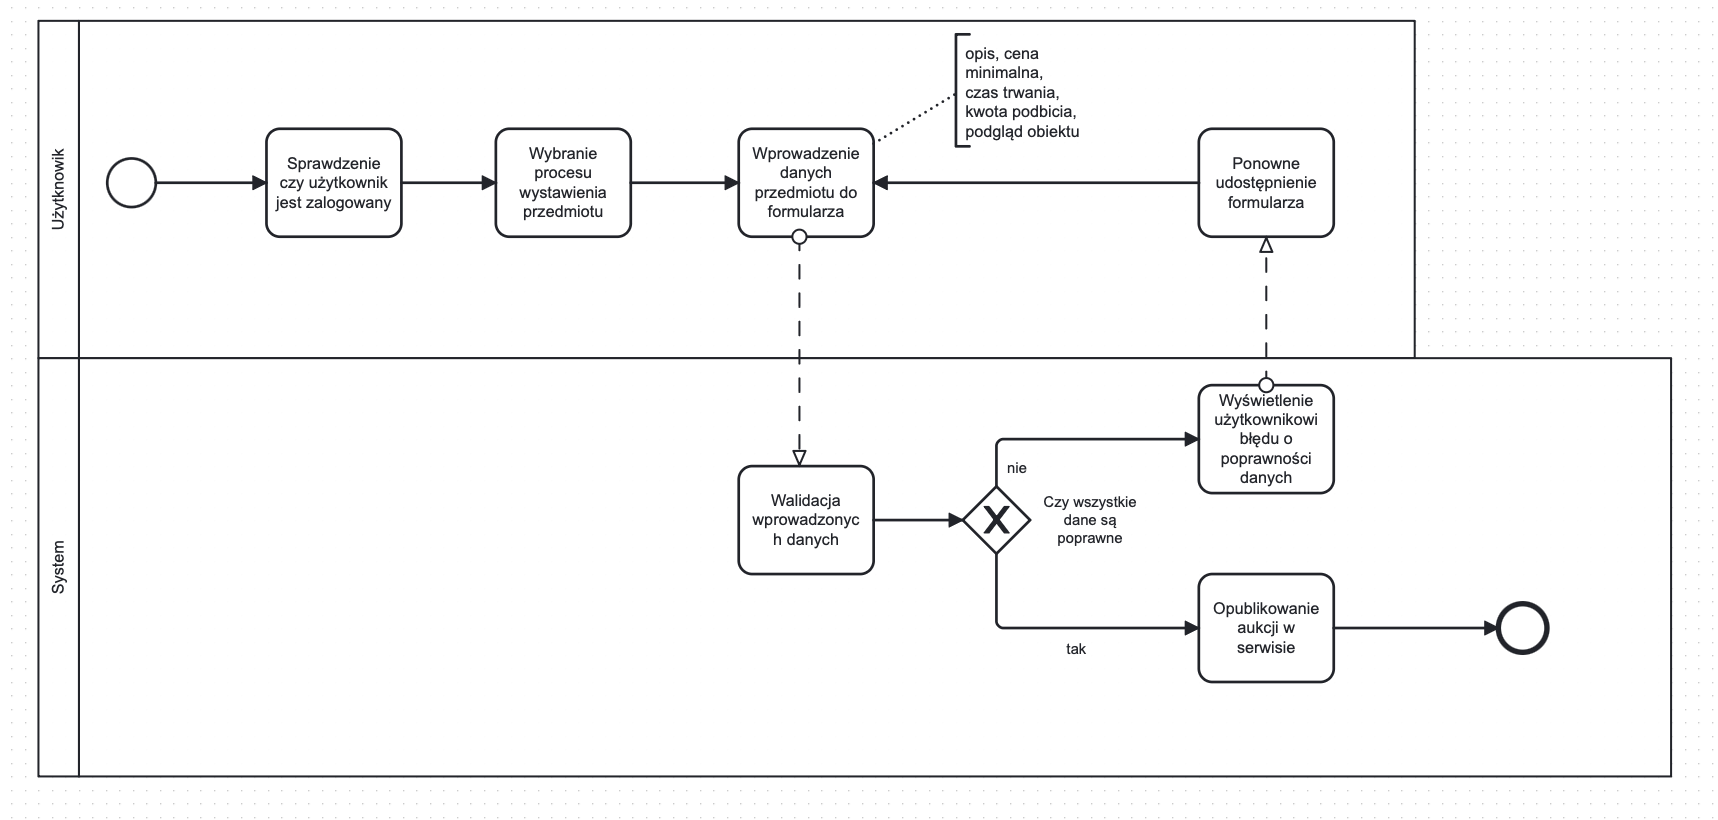
\includegraphics[width=\linewidth]{img/schematy/tworzenie aukcji.png}
    \captionof{figure}{Tworzenie aukcji}
    \label{fig:tworzenie_aukcji}
\end{center}
%\image{img/schematy/tworzenie aukcji.png}{Tworzenie aukcji}
\image{img/schematy/proces licytacji.png}{Proces licytacji}
\image{img/schematy/konczenie aukcji.png}{Kończenie aukcji}

\todo[inline]{Czy diagramy nie za małe? Można użyć \texttt{\textbackslash landscape}, ale czy w pracy można to zastosować?}

\subsection{Wymagania funkcjonalne:}
\begin{itemize}
    \item Obsługa aukcji
          \begin{itemize}
              \item System musi umożliwiać tworzenie i zarządzanie aukcjami przez zarejestrowane domy aukcyjne (zakres: kreacja, edycja, usuwanie aukcji).
              \item Każda aukcja powinna posiadać ustalony czas rozpoczęcia i zakończenia, automatyczne otwieranie i zamykanie zgodnie z harmonogramem.
              \item System musi zbierać i prezentować kluczowe parametry aukcji (status, cena wywoławcza, aktualna najwyższa oferta).
          \end{itemize}
    \item System licytacji w czasie rzeczywistym
          \begin{itemize}
              \item Użytkownicy powinni móc składać oferty online w trybie rzeczywistym, z mechanizmem aktualizacji najwyższej kwoty dla wszystkich obserwatorów.
              \item Mechanizm obsługi przebijania ofert: każde nowe przebicie powinno być natychmiast komunikowane pozostałym uczestnikom.
              \item Logika rozstrzygania zwycięzcy oraz rezerwacja przedmiotu po zakończeniu aukcji.
          \end{itemize}
    \item Wizualizacja 3D
          \begin{itemize}
              \item Dla każdej pozycji aukcyjnej system zapewnia podgląd modelu 3D przedmiotu, osadzony w interaktywnym viewerze.
              \item Viewer 3D powinien obsługiwać podstawowe operacje (obrót, przybliżenie/oddalenie), by użytkownik mógł dokładnie obejrzeć szczegóły oferty.
              \item Integracja procesu uploadu i weryfikacji pliku 3D w formatach ustalonych w specyfikacji technicznej.
          \end{itemize}
    \item Zarządzanie użytkownikami
          \begin{itemize}
              \item Rejestracja i uwierzytelnianie: tworzenie kont z walidacją danych, logowanie, wylogowanie, procedura resetu hasła.
              \item Konta użytkowników z podziałem na role: licytujący, dom aukcyjny, administrator. Każda rola ma inne uprawnienia (np. tylko dom aukcyjny może tworzyć aukcje).
              \item Profil użytkownika: edycja danych osobowych, podgląd historii aktywności (aukcje wygrane/przegrane, złożone oferty).
          \end{itemize}
    \item Interaktywna wyszukiwarka i filtry
          \begin{itemize}
              \item System wyszukiwania musi obsługiwać pełnotekstowe zapytania, filtrowanie wyników po parametrach (kategoria, przedział cenowy, status aukcji, dom aukcyjny itp.).
              \item Sortowanie wyników według różnych kryteriów (cena rosnąco/maleją\-co, najbliższe zakończenie, najnowsze).
              \item Możliwość zapamiętywania i zarządzania własnymi zestawami filtrów (ulubione kategorie, alerty o nowych aukcjach).
          \end{itemize}
\end{itemize}

\subsection{Wymagania niefunkcjonalne:}
\begin{itemize}
    \item Wydajność
          \begin{itemize}
              \item System musi gwarantować płynne renderowanie modeli 3D przy wykorzystaniu WebGPU, zapewniając interaktywność bez opóźnień.
              \item Prawidłowa optymalizacja strony pod względem dodawania treści.
              \item Ogólna skalowalność strony. System powinien pozwalać na obsługiwanie rosnącej liczby użytkowników na aukcji, przy zachowaniu wysokiej wydajności.
          \end{itemize}
\end{itemize}
\begin{itemize}
    \item Rozszerzalność i utrzymanie platformy
          \begin{itemize}
              \item Budowa systemu umożliwiająca dodawanie nowych funkcjonalności bez konieczności przebudowy całego systemu.
              \item Przejrzysta dokumentacja kodu i architektury, ułatwiająca przyszłe modyfikacje i integrację z innymi systemami.
          \end{itemize}
\end{itemize}
\begin{itemize}
    \item Użyteczność
          \begin{itemize}
              \item Intuicyjny, przejrzysty i klarowny dla użytkownika interfejs ułatwiający poruszanie się po serwisie zarówno dla strony kupującej jak i sprzedającej.
              \item Wsparcie dla nowoczesnych przeglądarek obsługujących WebGPU.
              \item Kompatybilność systemu dla wszystkich urządzeń.
          \end{itemize}
\end{itemize}

\subsection{Diagram pakietów przypadków użycia}
\begin{center}
    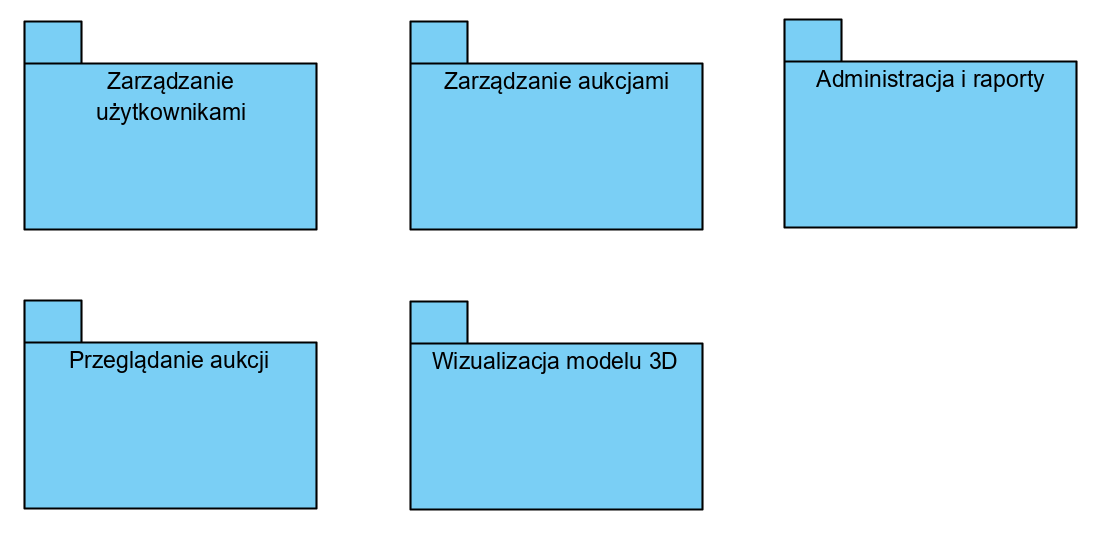
\includegraphics[width=\linewidth]{img/schematy/Diagram pakietow.png}
    \captionof{figure}{Diagram pakietów}
    \label{fig:diagram_pakietow}
\end{center}

\subsection{Diagramy przypadków użycia}
\begin{center}
    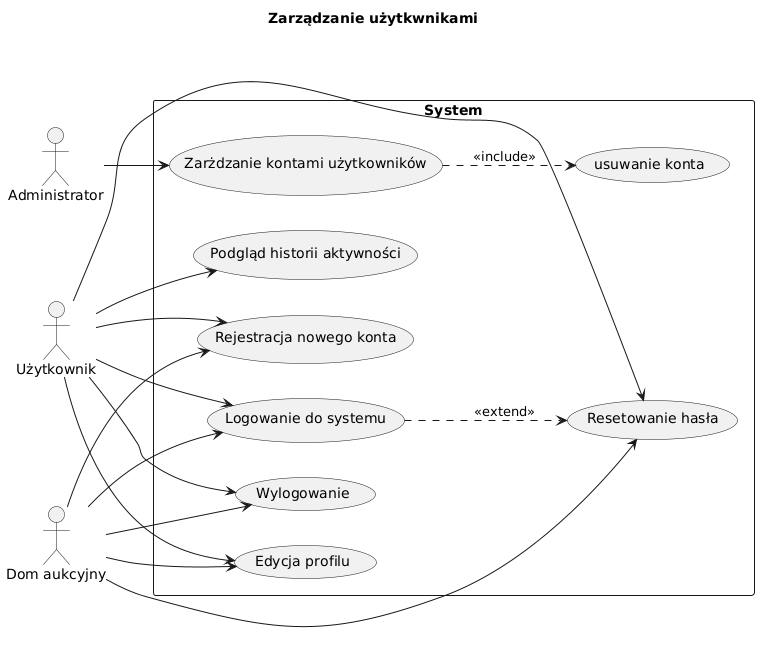
\includegraphics[width=\linewidth]{img/schematy/zarzadzanie-uzytkownikami.png}
    \captionof{figure}{Zarządzanie użytkownikami}
    \label{fig:diagram_przypadkow_uzycia}
\end{center}
%\image{img/schematy/zarzadzanie-uzytkownikami.png}{Zarządzanie użytkownikami}

\begin{figure}[htbp]
    \centering
    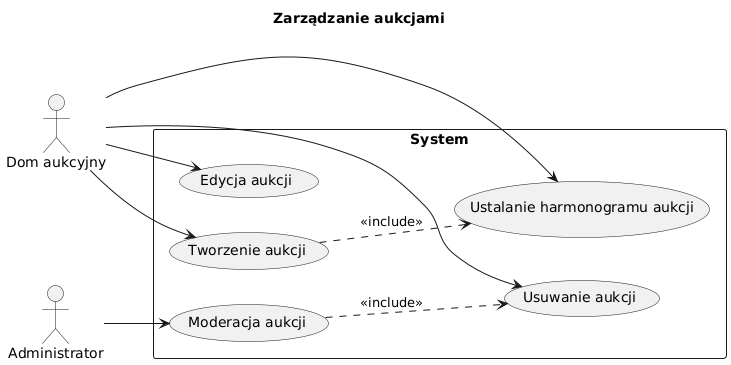
\includegraphics[
        width=\dimexpr\textwidth\relax,
        keepaspectratio
    ]{img/schematy/zarzadzanie-aukcjami.png}
    \caption{Zarządzanie aukcjami}
    \label{fig:zdj6}
\end{figure}

\begin{figure}[htbp]
    \centering
    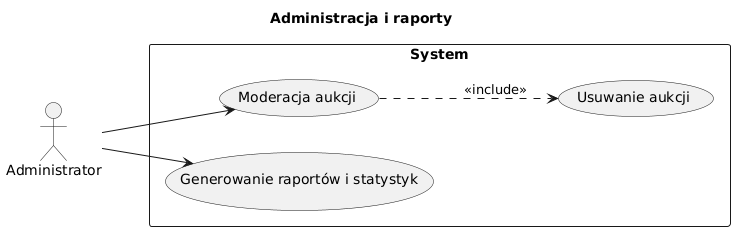
\includegraphics[
        width=\dimexpr\textwidth\relax,
        keepaspectratio
    ]{img/schematy/administracja-i-raporty.png}
    \caption{administracja i raporty}
    \label{fig:zdj7}
\end{figure}

\begin{figure}[htbp]
    \centering
    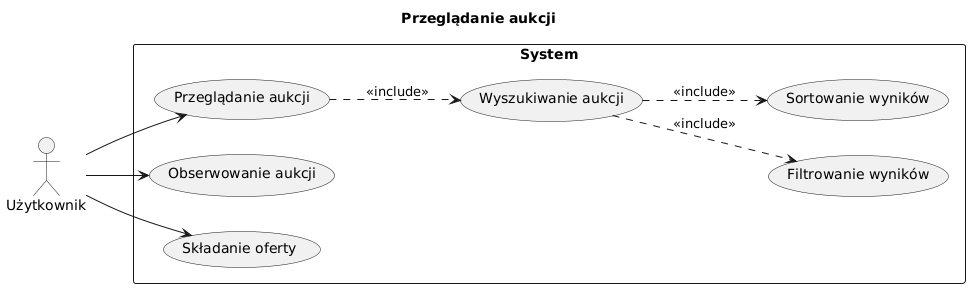
\includegraphics[
        width=\dimexpr\textwidth\relax,
        keepaspectratio
    ]{img/schematy/przegladanie-aukcji.png}
    \caption{Przeglądanie aukcji}
    \label{fig:zdj8}
\end{figure}

\begin{figure}[htbp]
    \centering
    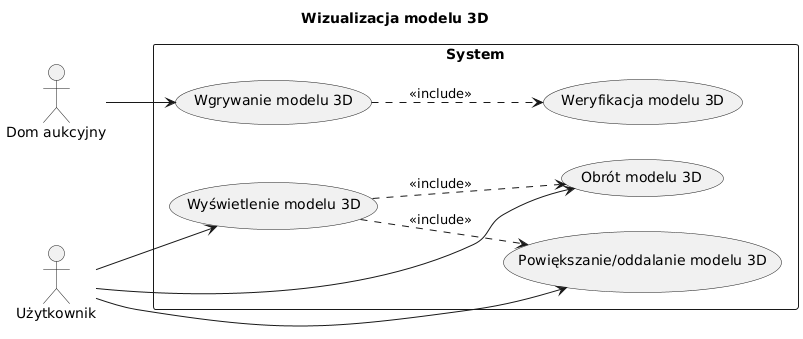
\includegraphics[
        width=\dimexpr\textwidth\relax,
        keepaspectratio
    ]{img/schematy/wizualizacja-3d.png}
    \caption{Wizualizacja modelu 3D}
    \label{fig:zdj9}
\end{figure}

\subsection{Historyjki użytkownika}
\subsubsection{Użytkownik}
\begin{itemize}
    \item \textbf{Jako} użytkownik,\\
          \textbf{Chciałbym} mieć podgląd przedmiotu w 3D, który wybrałem,\\
          \textbf{Aby} móc ocenić stan przedmiotu.\\
          \textbf{Zakładając}, że aukcja zawiera załadowany model 3D, \\
          \textbf{Jeśli} użytkownik kliknie przycisk „Podgląd 3D” na stronie aukcji, \\
          \textbf{To wtedy} interaktywny widok 3D przedmiotu zostanie wyświetlony.\\

    \item \textbf{Jako} użytkownik,\\
          \textbf{Chciałbym} móc obracać, przybliżać i oddalać przedmiot w podglądzie 3D,\\
          \textbf{Aby} móc dokładniej ocenić stan przedmiotu.\\
          \textbf{Zakładając}, że widoczny jest model 3D w viewerze,\\
          \textbf{Jeśli} użytkownik użyje myszy lub gestów dotykowych,\\
          \textbf{To wtedy} model zareaguje odpowiednio na obrót, przybliżenie i oddalenie.\\


    \item \textbf{Jako} użytkownik,\\
          \textbf{Chciałbym} w czasie rzeczywistym móc licytować wybrany przedmiot,\\
          \textbf{Aby} dokonać jego zakupu.\\
          \textbf{Zakładając}, że użytkownik jest zalogowany i aukcja jest aktywna,\\
          \textbf{Jeśli} wpisze ofertę wyższą niż obecna i kliknie „Licytuj”,\\
          \textbf{To wtedy} jego oferta stanie się najwyższą i będzie widoczna dla innych w czasie rzeczywistym.\\

    \item \textbf{Jako} użytkownik,\\
          \textbf{Chciałbym} móc wyszukać przedmiot, który mnie interesuje i wyświetlić 10 przedmiotów, które pasują do wyszukanego przedmiotu,\\
          \textbf{Aby} mieć przedmioty do porównania.\\
          \textbf{Zakładając}, że użytkownik wpisze zapytanie w wyszukiwarce,\\
          \textbf{Jeśli} wyników jest więcej niż 10,\\
          \textbf{To wtedy} system wyświetli pierwsze 10 najbardziej dopasowanych aukcji do zapytania.\\
    \item \textbf{Jako} użytkownik,\\
          \textbf{Chciałbym} móc zawęzić ilość wyszukanych przedmiotów przez zastosowanie filtrów ceny (filtrowanie według ceny malejąco i rosnąco),\\
          \textbf{Aby} wyrzucić przedmioty, które nie będą w moim budżecie \\
          \textbf{Zakładając}, że użytkownik określi przedział cenowy lub wybierze sortowanie po cenie,\\
          \textbf{Jeśli} kliknie „Zastosuj filtr”,\\
          \textbf{To wtedy} system pokaże tylko aukcje mieszczące się w wybranym przedziale lub odpowiednio posortowane.\\
    \item \textbf{Jako} użytkownik,\\
          \textbf{Chciałbym} móc zawęzić ilość wyszukanych przedmiotów przez zastosowanie filtrów czasowych licytacji (od najstarszego do najnowszego), \\
          \textbf{Aby} móc ominąć starsze licytacje.\\
          \textbf{Zakładając}, że użytkownik wybierze sortowanie według daty rozpoczęcia lub zakończenia aukcji,\\
          \textbf{Jeśli} kliknie „Zastosuj”,\\
          \textbf{To wtedy} system posortuje lub przefiltruje aukcje zgodnie z wybranym zakresem czasowym.\\
    \item \textbf{Jako} użytkownik,\\
          \textbf{Chciałbym} móc dodać przedmiot do sekcji obserwowane,\\
          \textbf{Aby} mieć przedmioty, które mnie interesują w jednej sekcji.\\
          \textbf{Zakładając}, że użytkownik jest zalogowany i przegląda aukcję,\\
          \textbf{Jeśli} kliknie ikonę „Dodaj do obserwowanych”,\\
          \textbf{To wtedy} przedmiot zostanie zapisany w sekcji „Obserwowane” na jego profilu.\\

    \item \textbf{Jako} użytkownik\\
          \textbf{Chciałbym} zobaczyć swoją historię zakupów, których dokonałem,\\
          \textbf{Aby} móc szybko wyszukać zakupiony przedmiot \\
          \textbf{Zakładając}, że użytkownik jest zalogowany,\\
          \textbf{Jeśli} przejdzie do swojego profilu i kliknie „Historia zakupów”,\\
          \textbf{To wtedy} system wyświetli listę wygranych przez niego aukcji.\\
\end{itemize}
\subsubsection{Administrator}
\begin{itemize}
    \item \textbf{Jako} administrator,\\
          \textbf{Chciałbym} móc moderować aukcje na platformie, \\
          \textbf{Aby} usuwać z serwisu nieodpowiednie oferty i zapewnić bezpieczeństwo użytkownikom. \\
          \textbf{Zakładając}, że istnieje aukcja zawierająca niedozwolone treści,\\
          \textbf{Jeśli} administrator wybierze opcję usunięcia tej aukcji, \\
          \textbf{To wtedy} aukcja zostanie trwale usunięta z systemu.\\
    \item \textbf{Jako} administrator, \\
          \textbf{Chciałbym} generować raporty i statystyki platformy \\
          \textbf{Aby} analizować aktywność użytkowników i wyniki aukcji. \\
          \textbf{Zakładając}, że system posiada dane o aukcjach i użytkownikach,\\
          \textbf{Jeśli} administrator wybierze zakres dat i kliknie „Generuj raport”,\\
          \textbf{To wtedy} system przedstawi zestawienie z wykresami lub tabelami odzwierciedlającymi statystyki (np. liczbę aukcji, wartość licytacji, liczbę aktywnych użytkowników).


\end{itemize}
\subsubsection{Dom aukcyjny}
\begin{itemize}
    \item \textbf{Jako} dom aukcyjny,\\
          \textbf{Chciałbym} zarejestrować konto w serwisie \\
          \textbf{Aby} móc tworzyć i wystawiać własne aukcje:\\
          \textbf{Zakładając}, że podano prawidłowe dane rejestracyjne (w tym informacje o domu aukcyjnym),\\
          \textbf{Jeśli} formularz rejestracji zostanie poprawnie wypełniony i zatwierdzony,\\
          \textbf{To wtedy} konto domu aukcyjnego zostanie utworzone, a użytkownik uzyska dostęp do panelu aukcyjnego.\\



    \item \textbf{Jako} dom aukcyjny,\\
          \textbf{Chciałbym} wystawiać nowe aukcje ze szczegółowym opisem i modelami 3D przedmiotów \\
          \textbf{Aby} prezentować oferowane przedmioty w atrakcyjny sposób potencjalnym klientom\\
          \textbf{Zakładając}, że jestem zalogowany jako dom aukcyjny i mam wszystkie dane przedmiotu (opis, zdjęcia, model 3D),\\
          \textbf{Jeśli} wypełnię formularz tworzenia aukcji i potwierdzę jego dodanie, \\
          \textbf{To wtedy} nowa aukcja pojawi się na liście dostępnych aukcji na platformie.
\end{itemize}

\todo[inline]{Pomysł: każda historyjka w oddzielone ramki za pomocą paczki tcolorbox lub innej.}

\subsection{Diagramy klas}
\todo[inline]{bez landscape obrazki bardzo nieczytelne}
\begin{landscape}
    \begin{figure}[p]
        \centering
        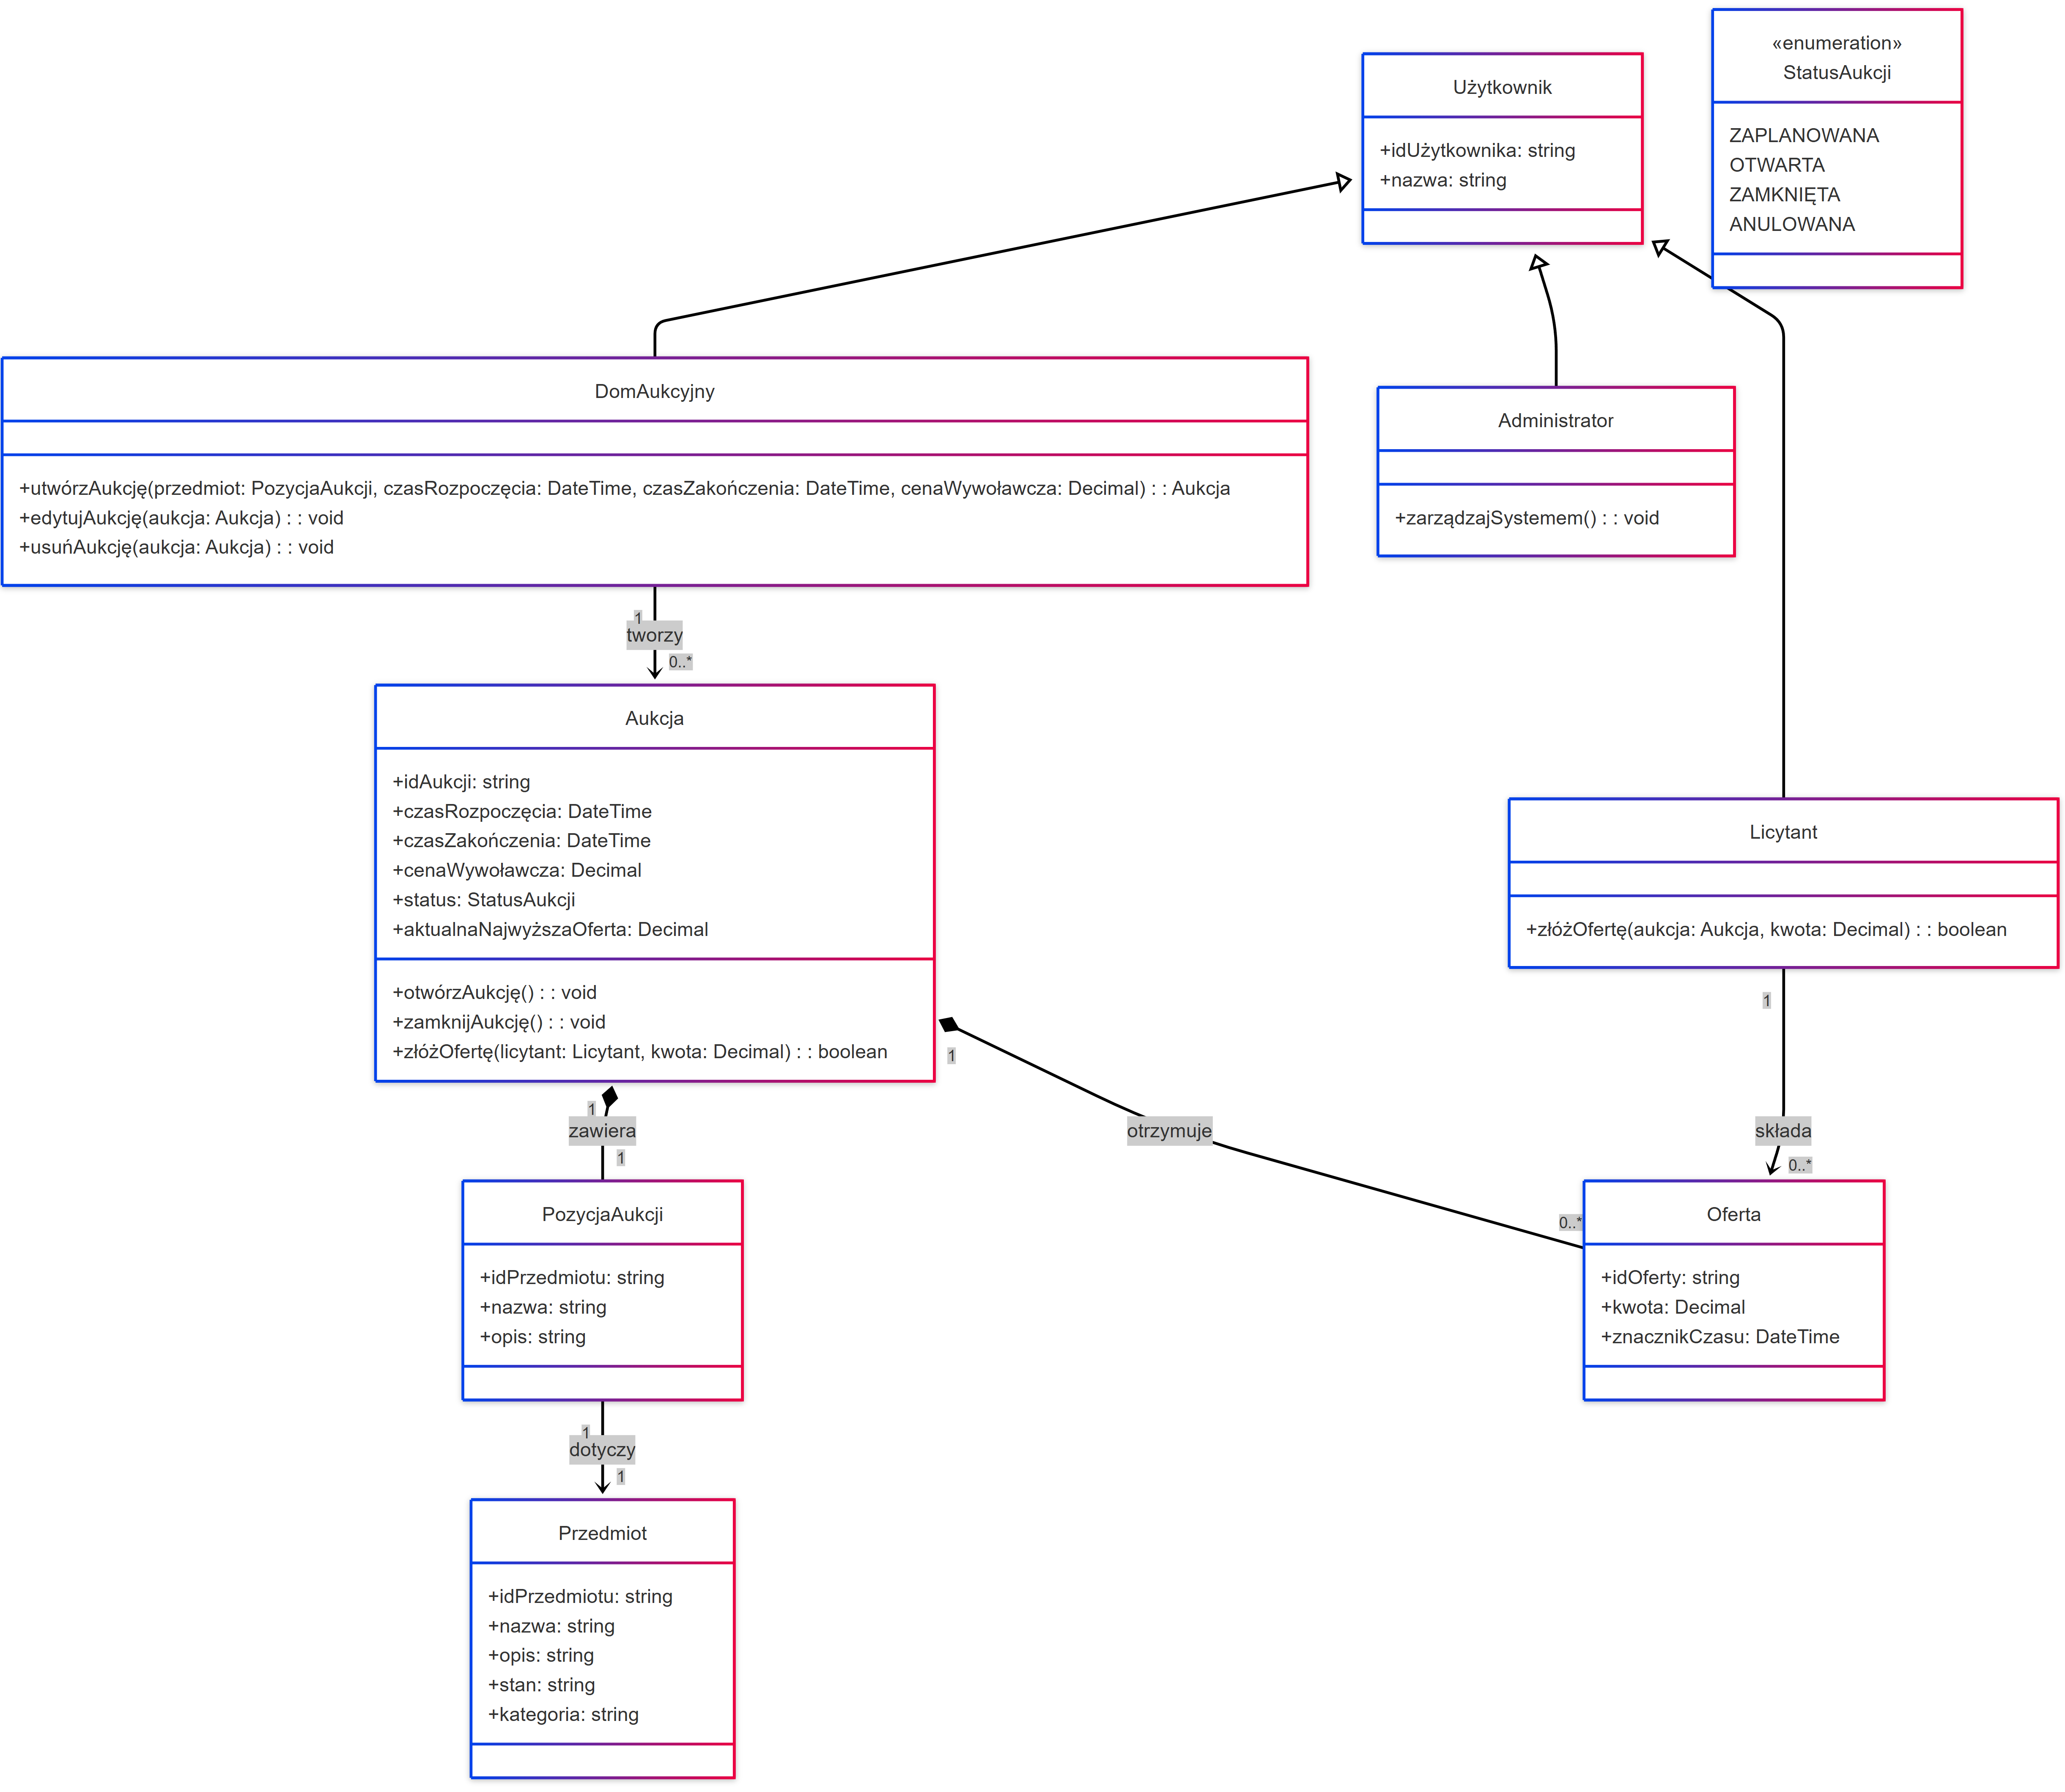
\includegraphics[
            width=\dimexpr\paperheight\relax,
            height=\dimexpr\textwidth\relax,
            keepaspectratio
        ]{img/schematy/proces-licytacji-CD.png}
        \caption{Proces licytacji}
        \label{fig:zdj10}
    \end{figure}

    \begin{figure}[p]
        \centering
        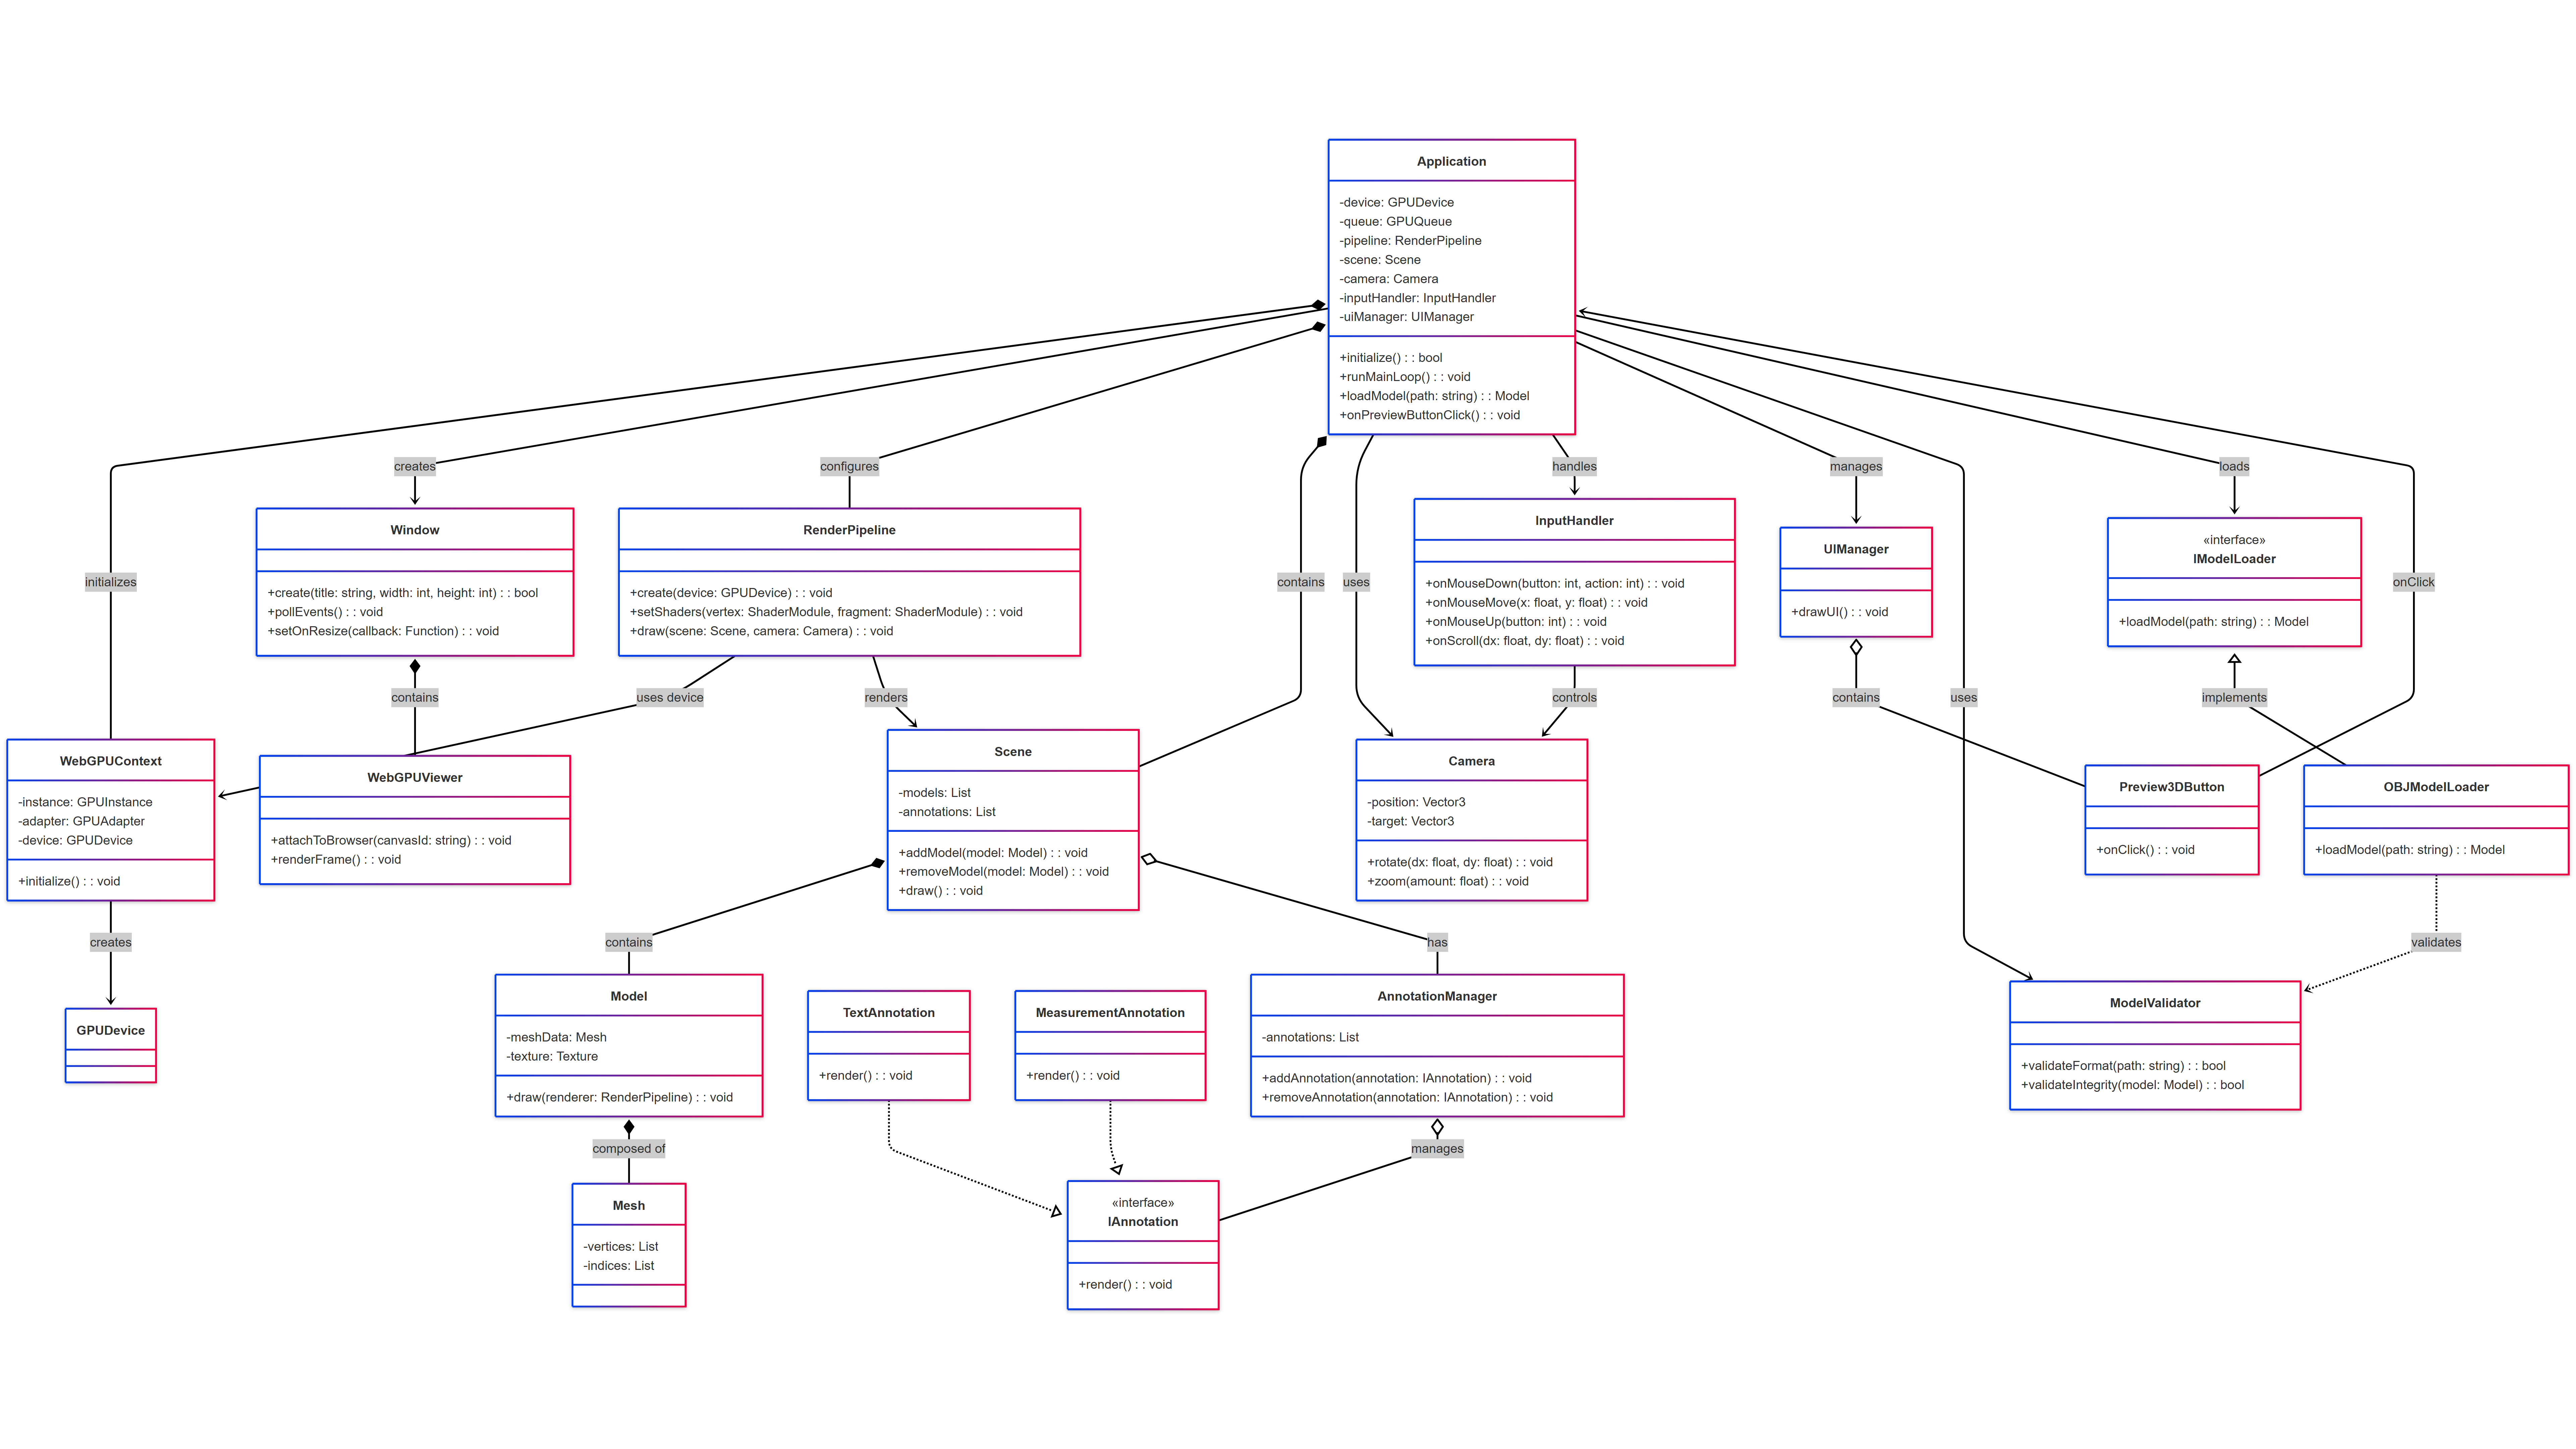
\includegraphics[
            width=\dimexpr\paperheight\relax,
            height=\dimexpr\textwidth\relax-67pt,
            keepaspectratio
        ]{img/schematy/wizualizacja-obiektu-CD.png}
        \caption{Wizualizacja obiektu 3D}
        \label{fig:zdj11}
    \end{figure}
\end{landscape}

\subsection{Diagramy sekwencji}
\begin{center}
    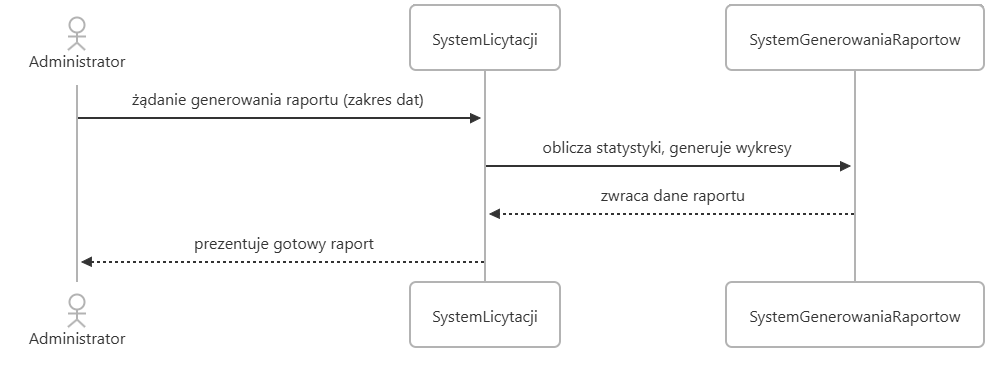
\includegraphics[width=\linewidth]{img/schematy/GenerowanieRaportow.png}
    \captionof{figure}{Generowanie raportów}
    \label{fig:generowanie_raportow}
\end{center}

\begin{figure}[htbp]
    \centering
    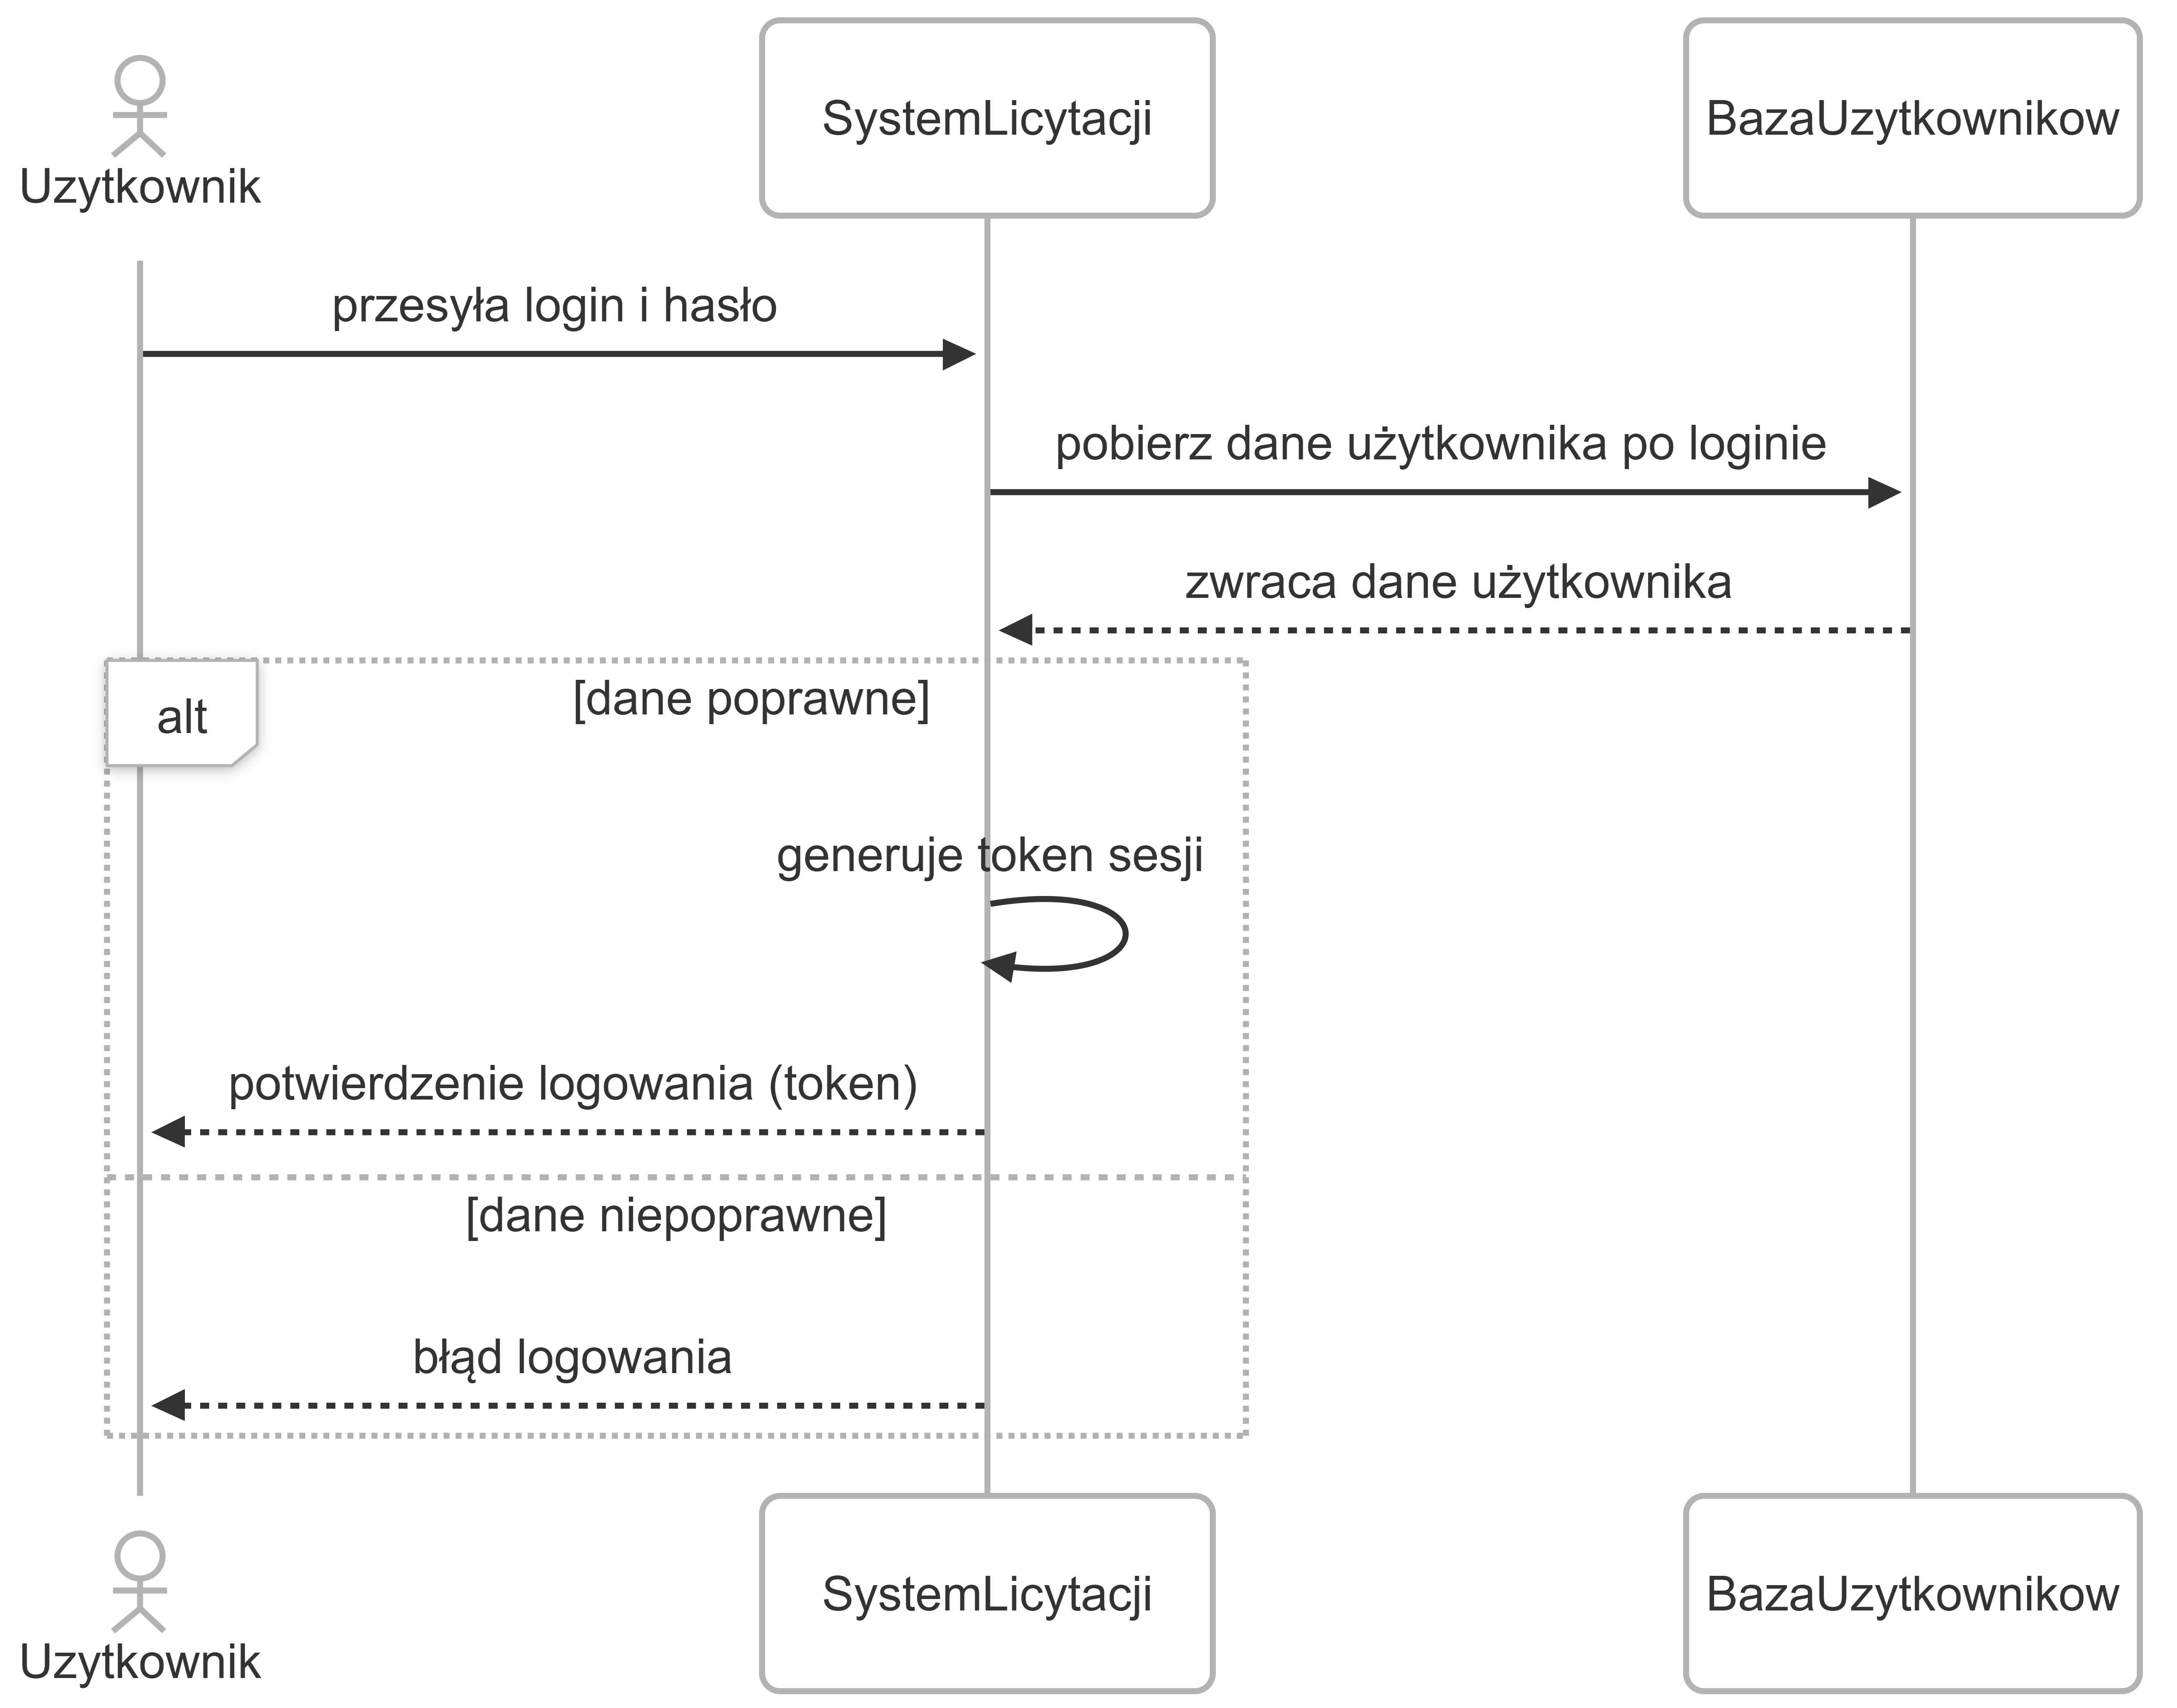
\includegraphics[
        width=\dimexpr\textwidth\relax,
        keepaspectratio
    ]{img/schematy/Logowanie.png}
    \caption{Logowanie}
    \label{fig:zdj13}
\end{figure}

\begin{figure}[htbp]
    \centering
    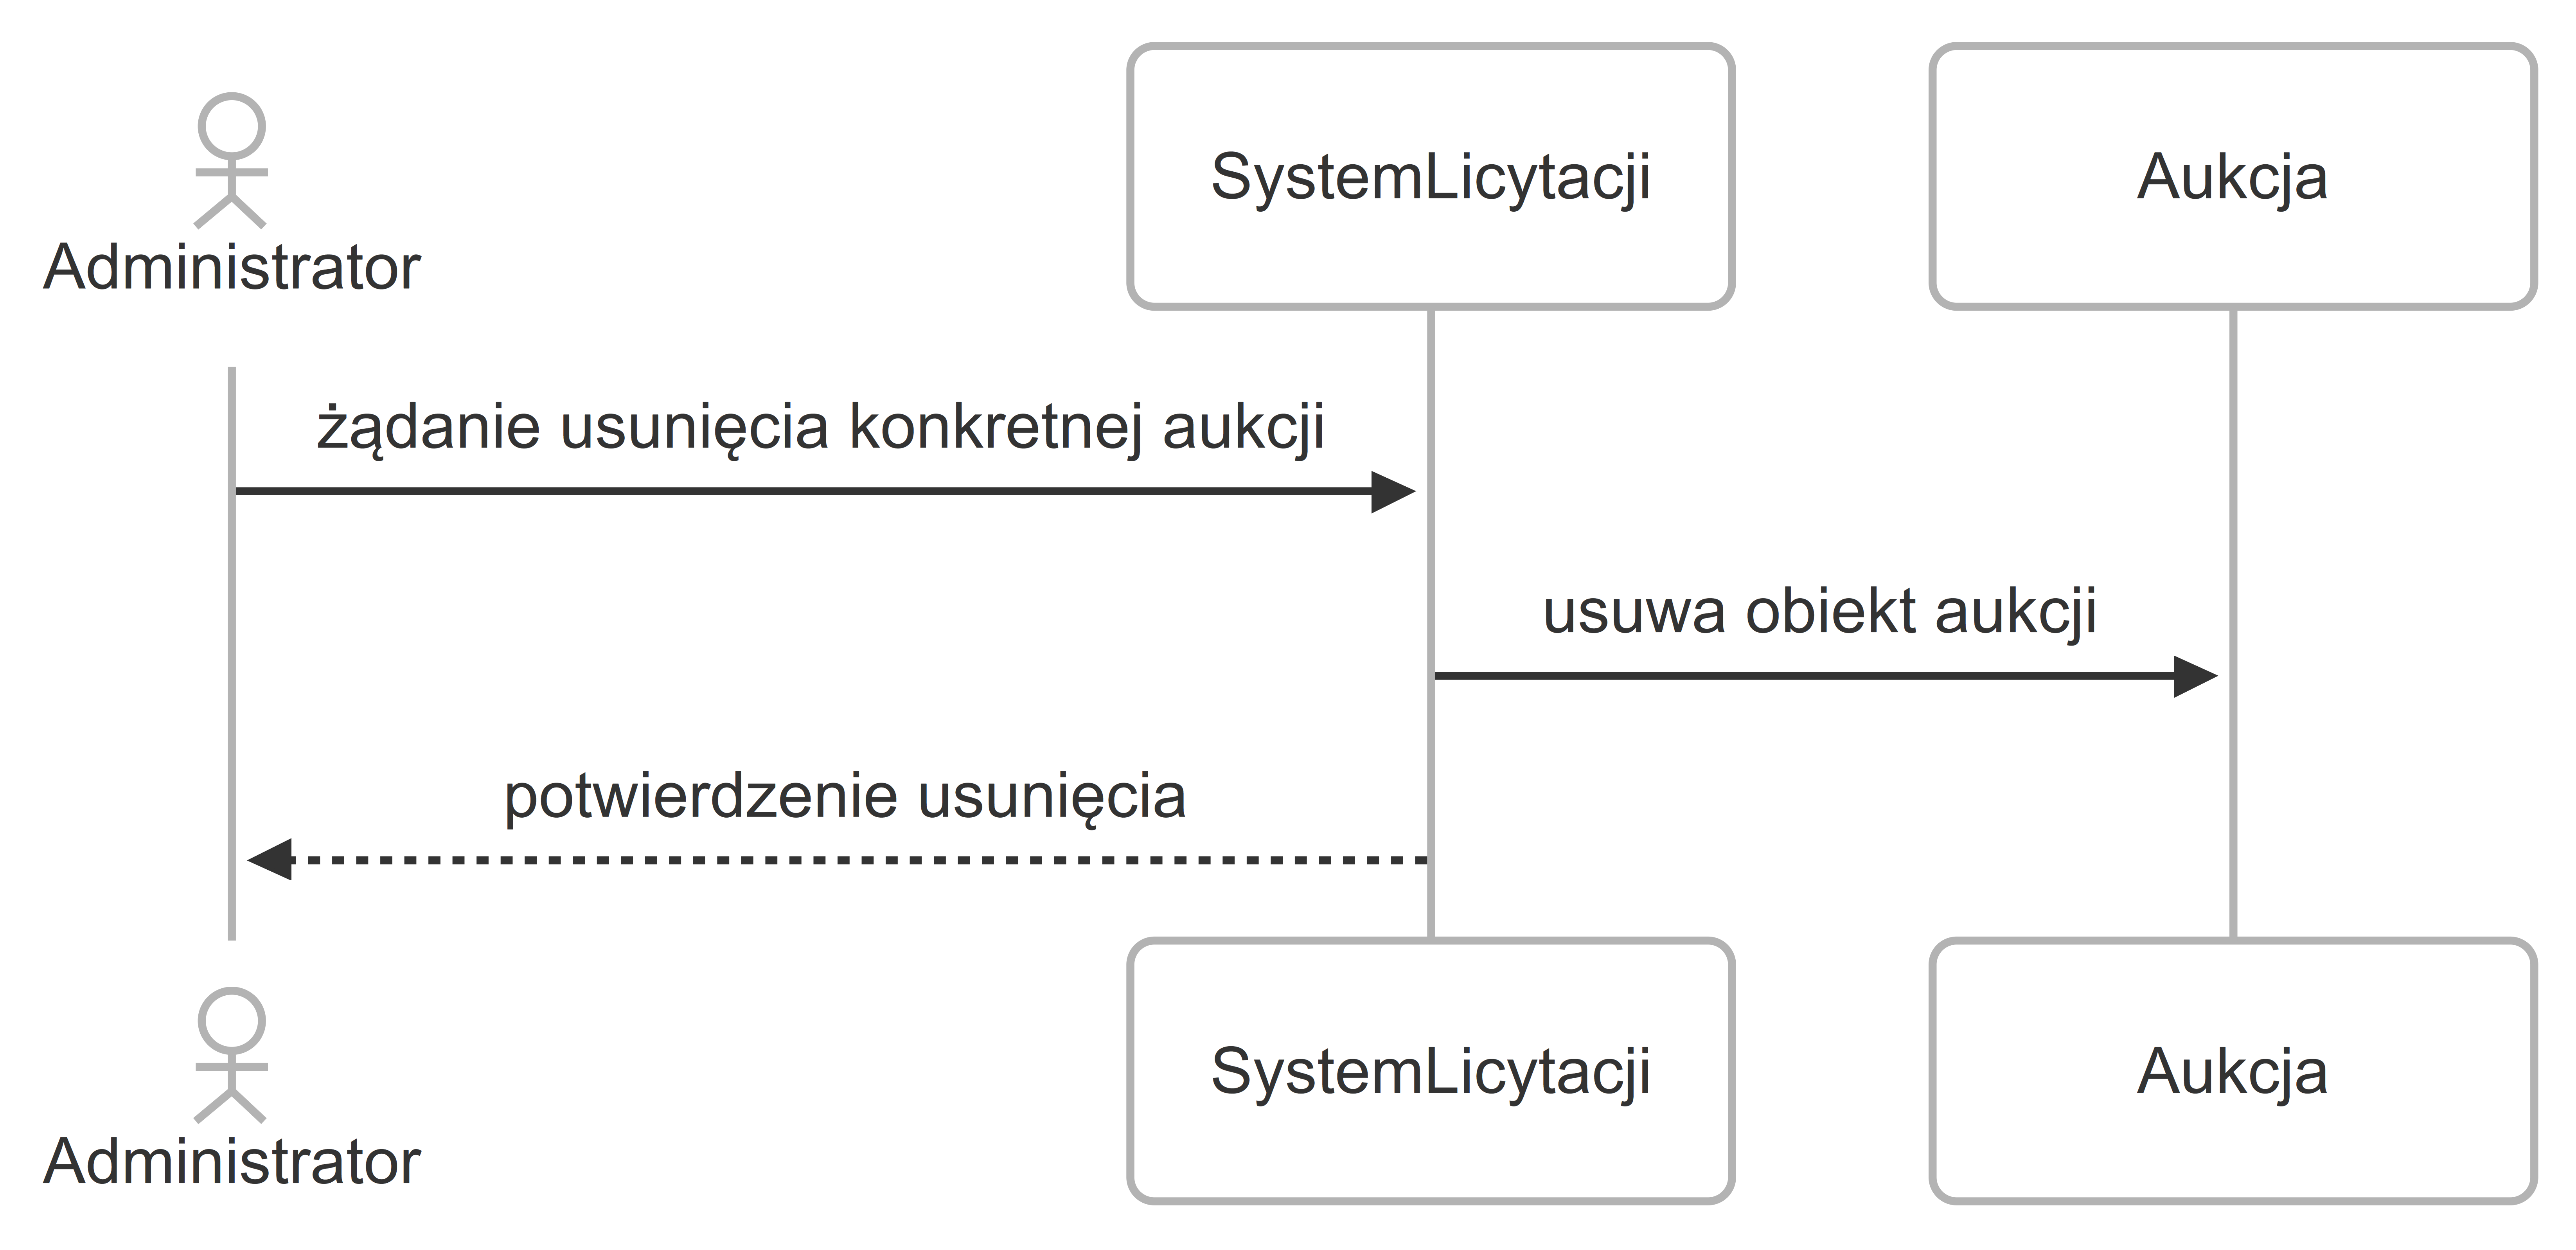
\includegraphics[
        width=\dimexpr\textwidth\relax,
        keepaspectratio
    ]{img/schematy/ModeracjaAukcji.png}
    \caption{Moderacja aukcji}
    \label{fig:zdj14}
\end{figure}

\begin{figure}[htbp]
    \centering
    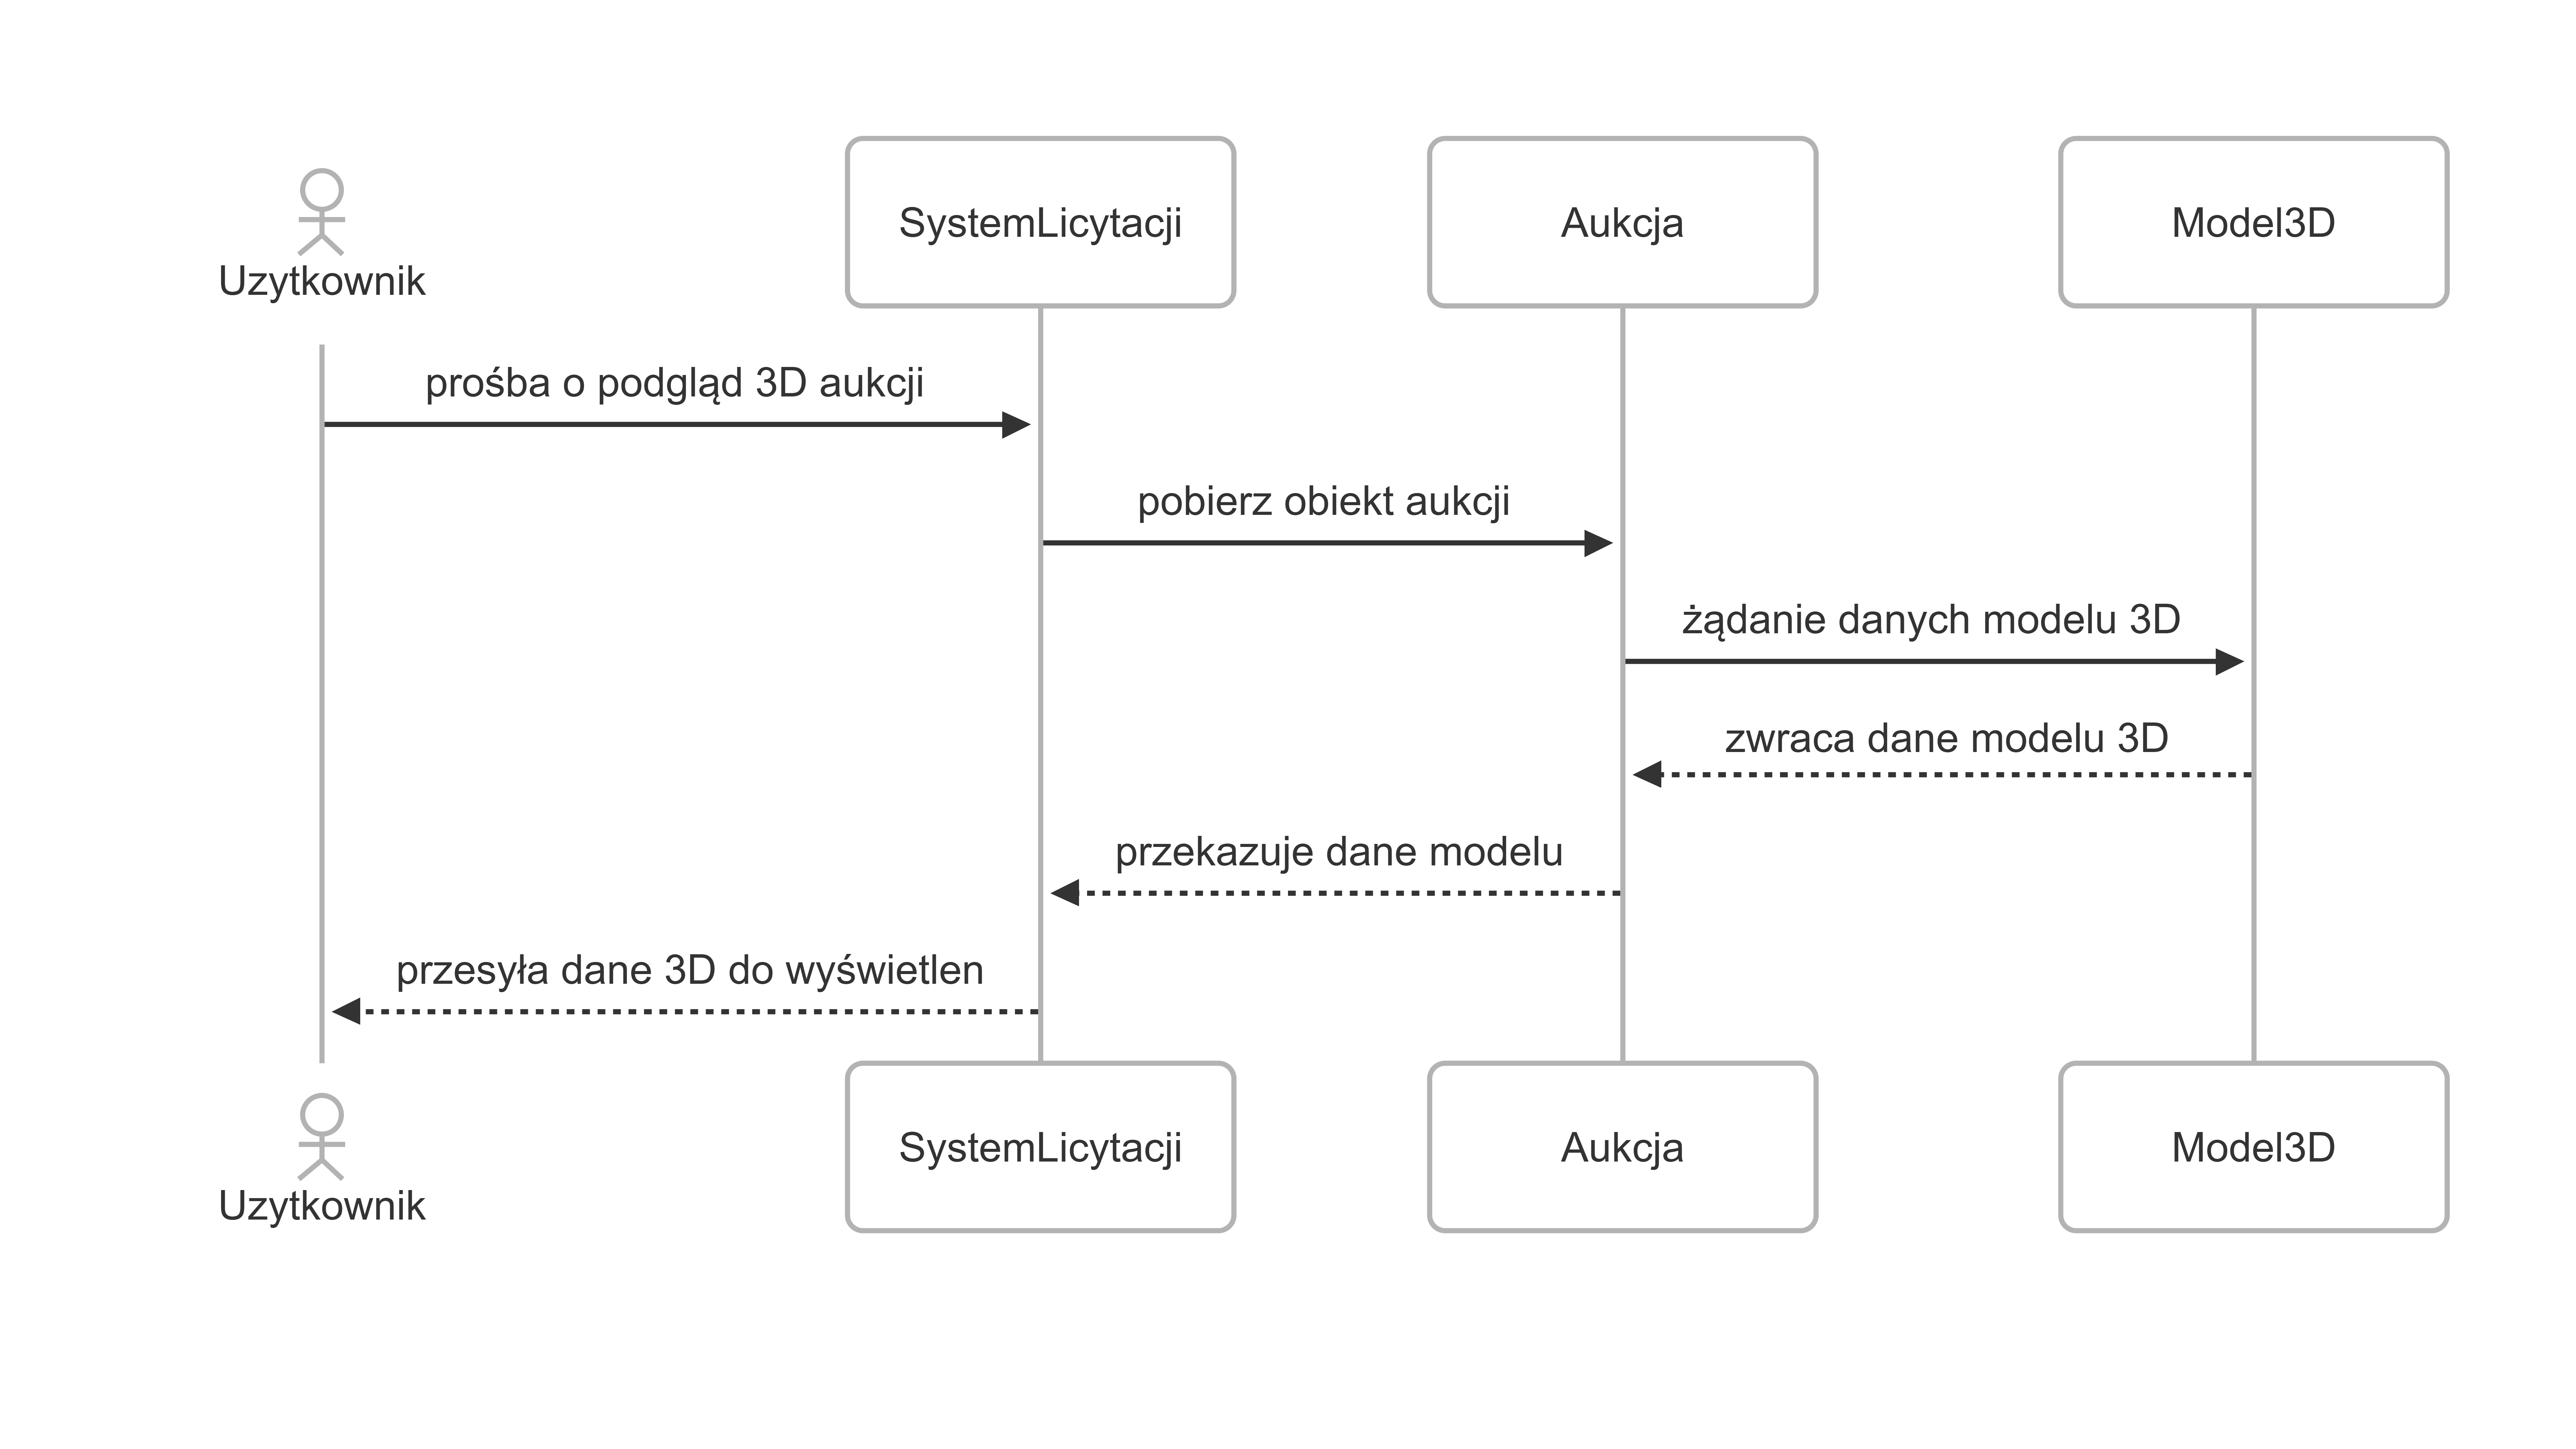
\includegraphics[
        width=\dimexpr\textwidth\relax,
        keepaspectratio
    ]{img/schematy/PodgladModelu3D.png}
    \caption{Wizualizacja modelu 3D}
    \label{fig:zdj15}
\end{figure}

\begin{figure}[htbp]
    \centering
    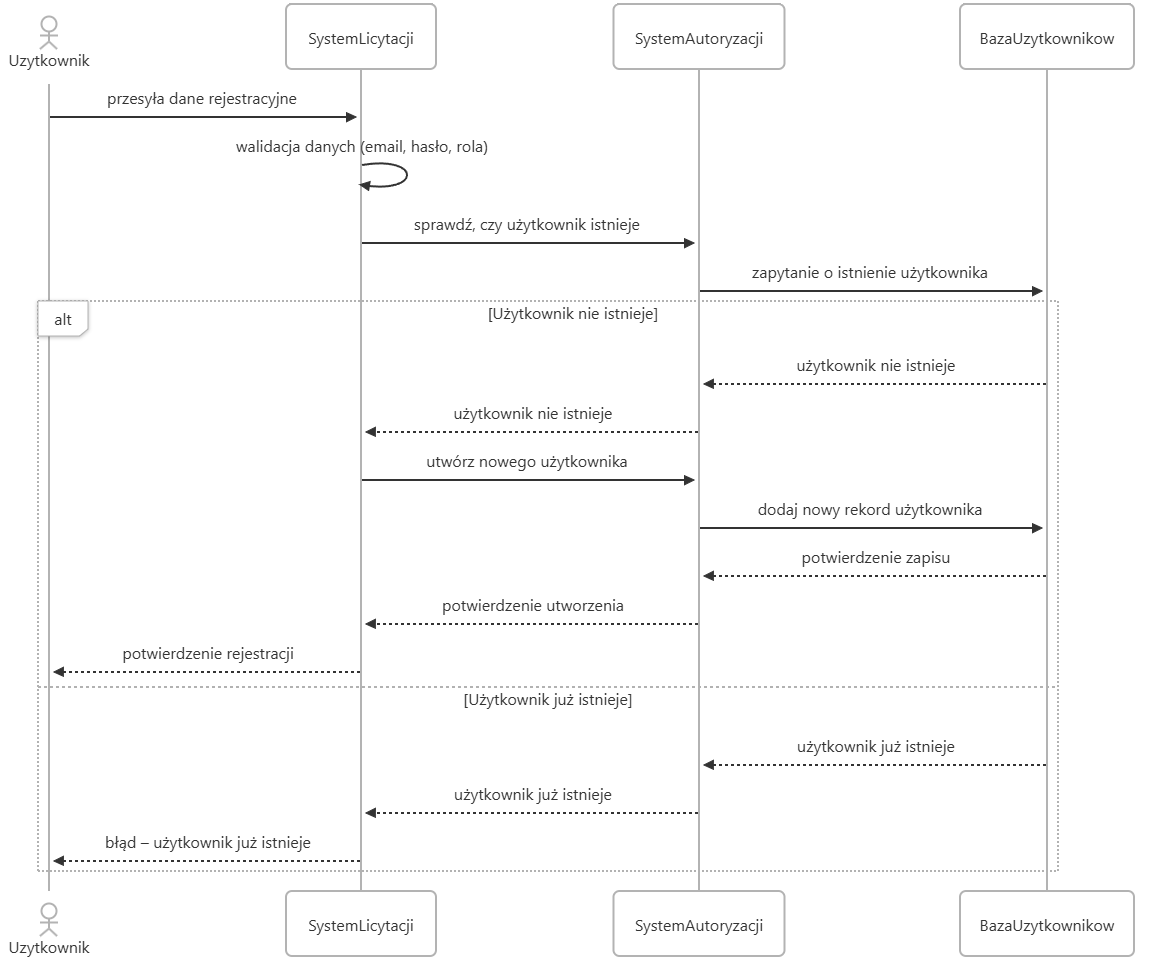
\includegraphics[
        width=\dimexpr\textwidth\relax,
        keepaspectratio
    ]{img/schematy/Rejestracja.png}
    \caption{Rejestracja}
    \label{fig:zdj16}
\end{figure}

\begin{figure}[htbp]
    \centering
    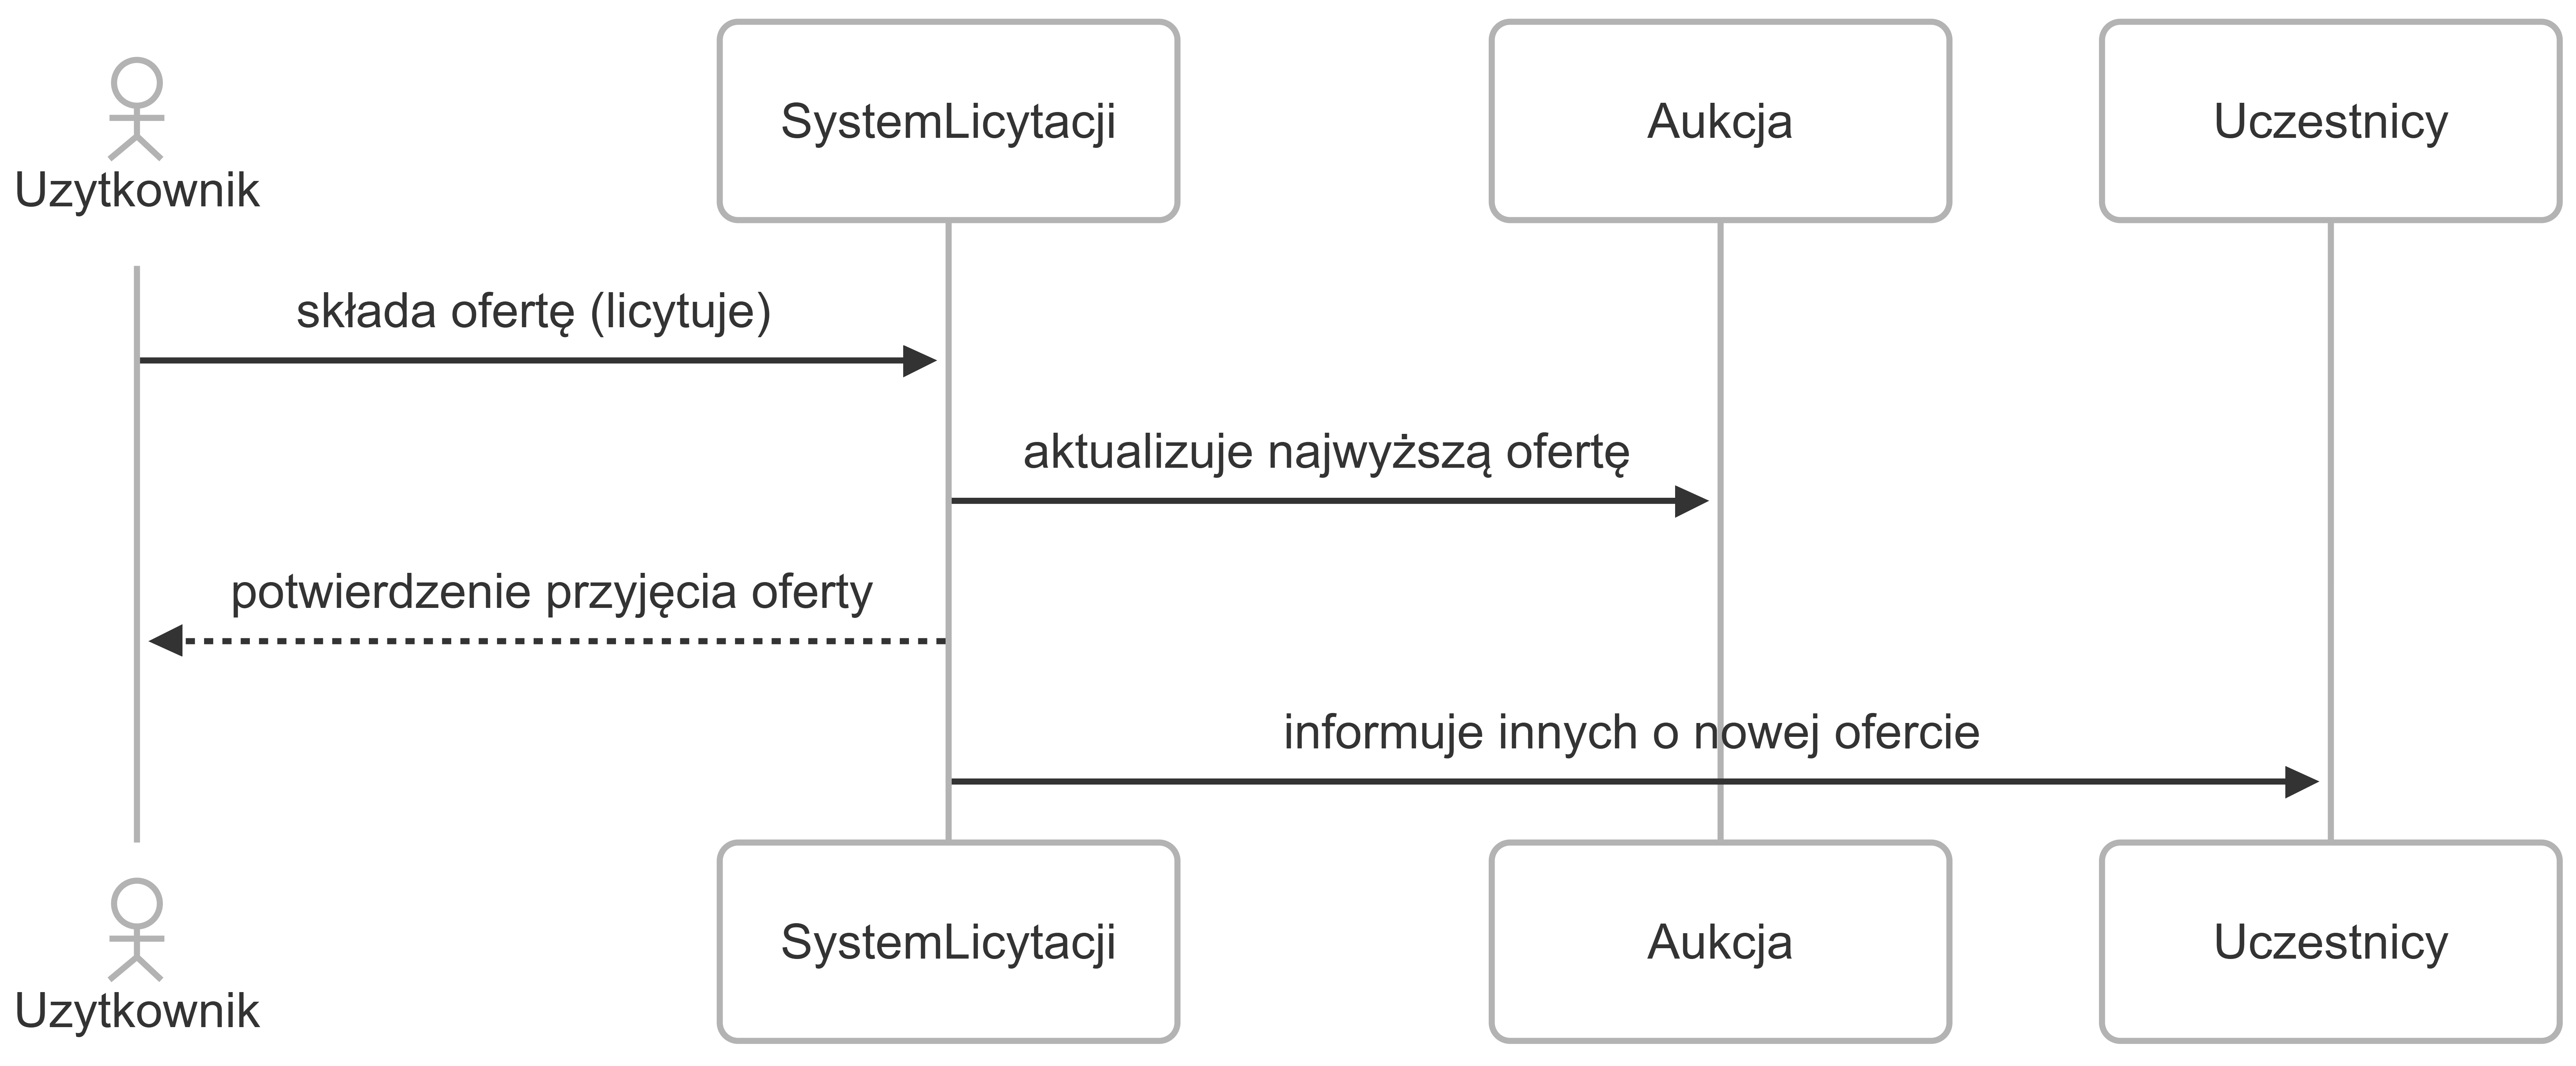
\includegraphics[
        width=\dimexpr\textwidth\relax,
        keepaspectratio
    ]{img/schematy/SystemLicytowania.png}
    \caption{System licytowania}
    \label{fig:zdj17}
\end{figure}

\begin{figure}[htbp]
    \centering
    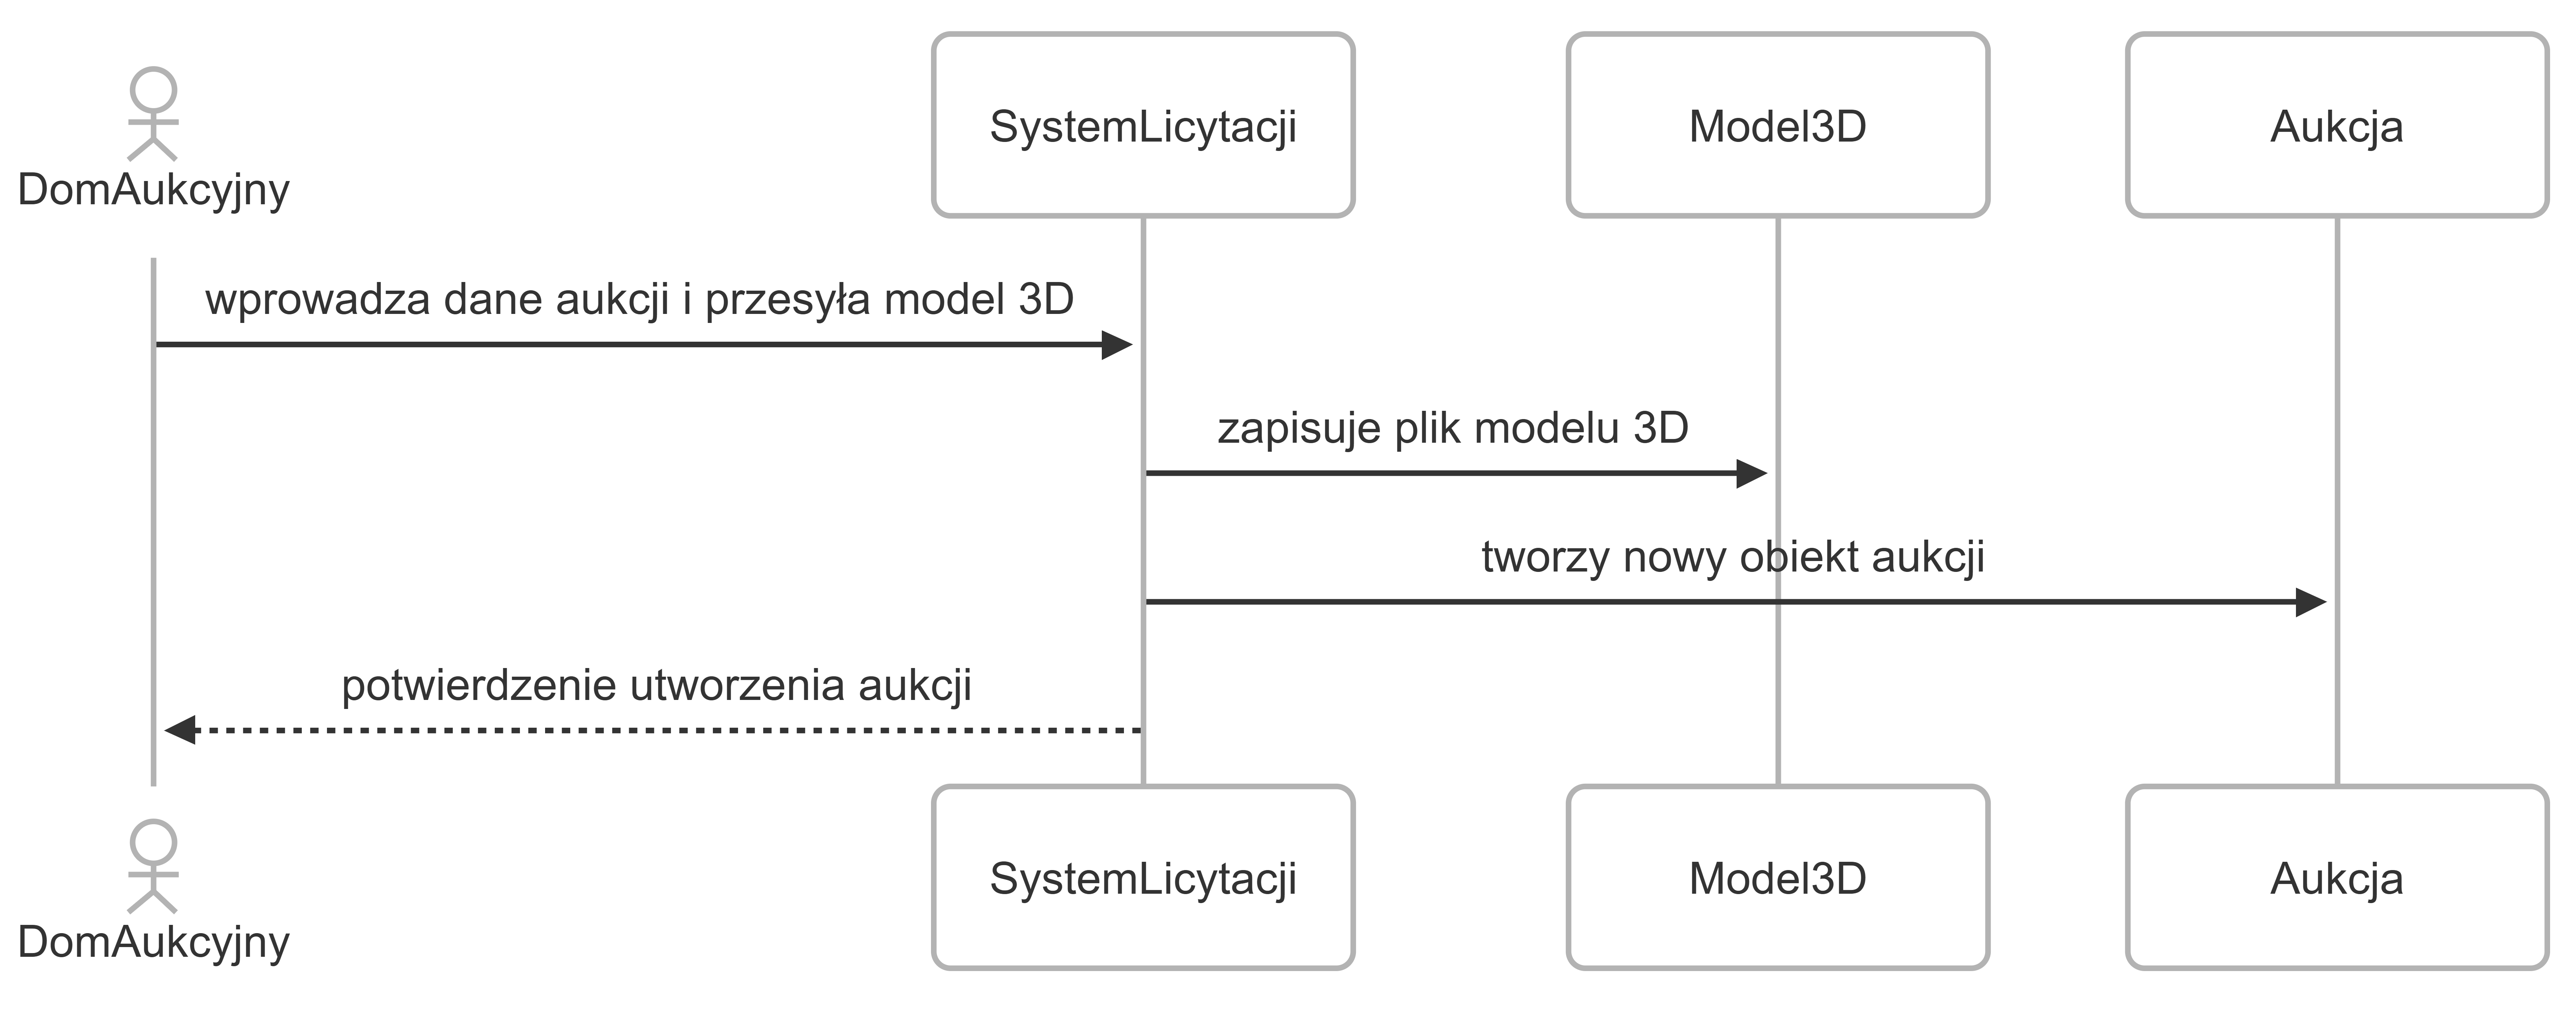
\includegraphics[
        width=\dimexpr\textwidth\relax,
        keepaspectratio
    ]{img/schematy/TworzenieAukcji.png}
    \caption{Tworzenie aukcji}
    \label{fig:zdj18}
\end{figure}

\subsection{Projekt interfejsu użytkownika}
\begin{landscape}
    \begin{figure}[p]
        \centering
        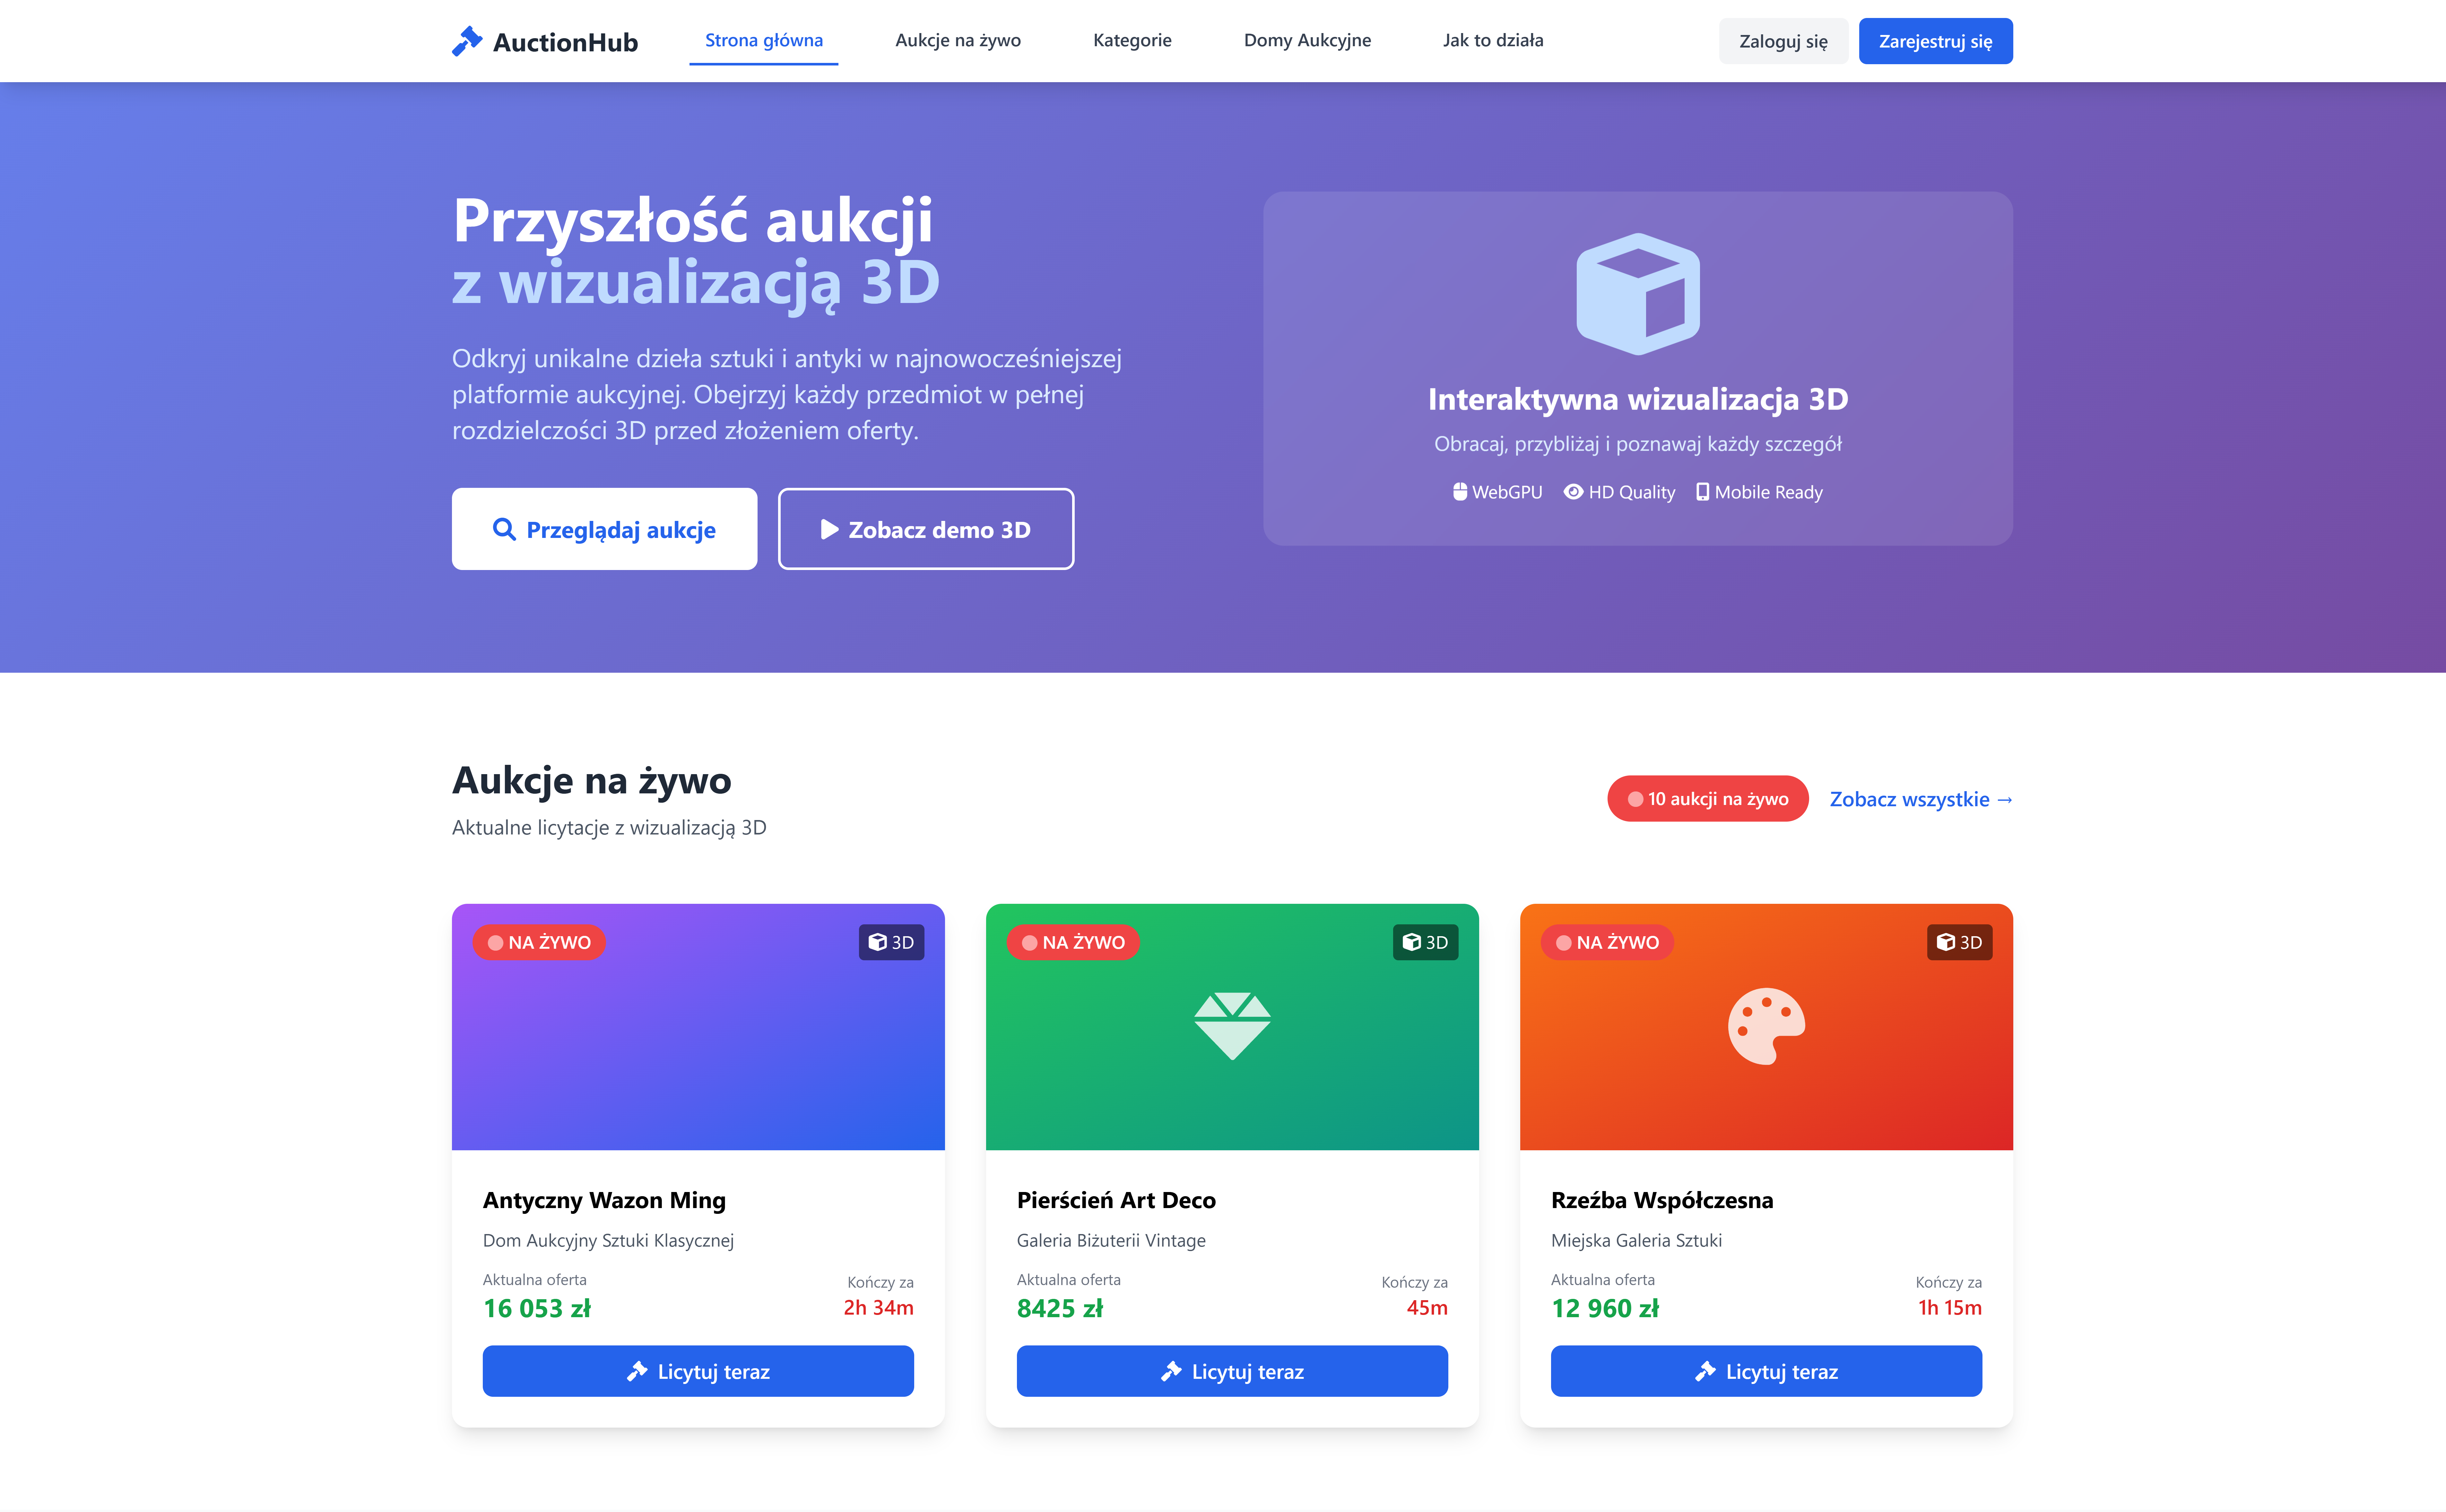
\includegraphics[
            width=\dimexpr\paperheight-2cm\relax,
            height=\dimexpr\textwidth-2cm\relax,
            keepaspectratio
        ]{img/schematy/mockup-strona-glowna-1.png}
        \caption{Mockup strony głównej - widok 1}
        \label{fig:mockup1}
    \end{figure}

    \begin{figure}[p]
        \centering
        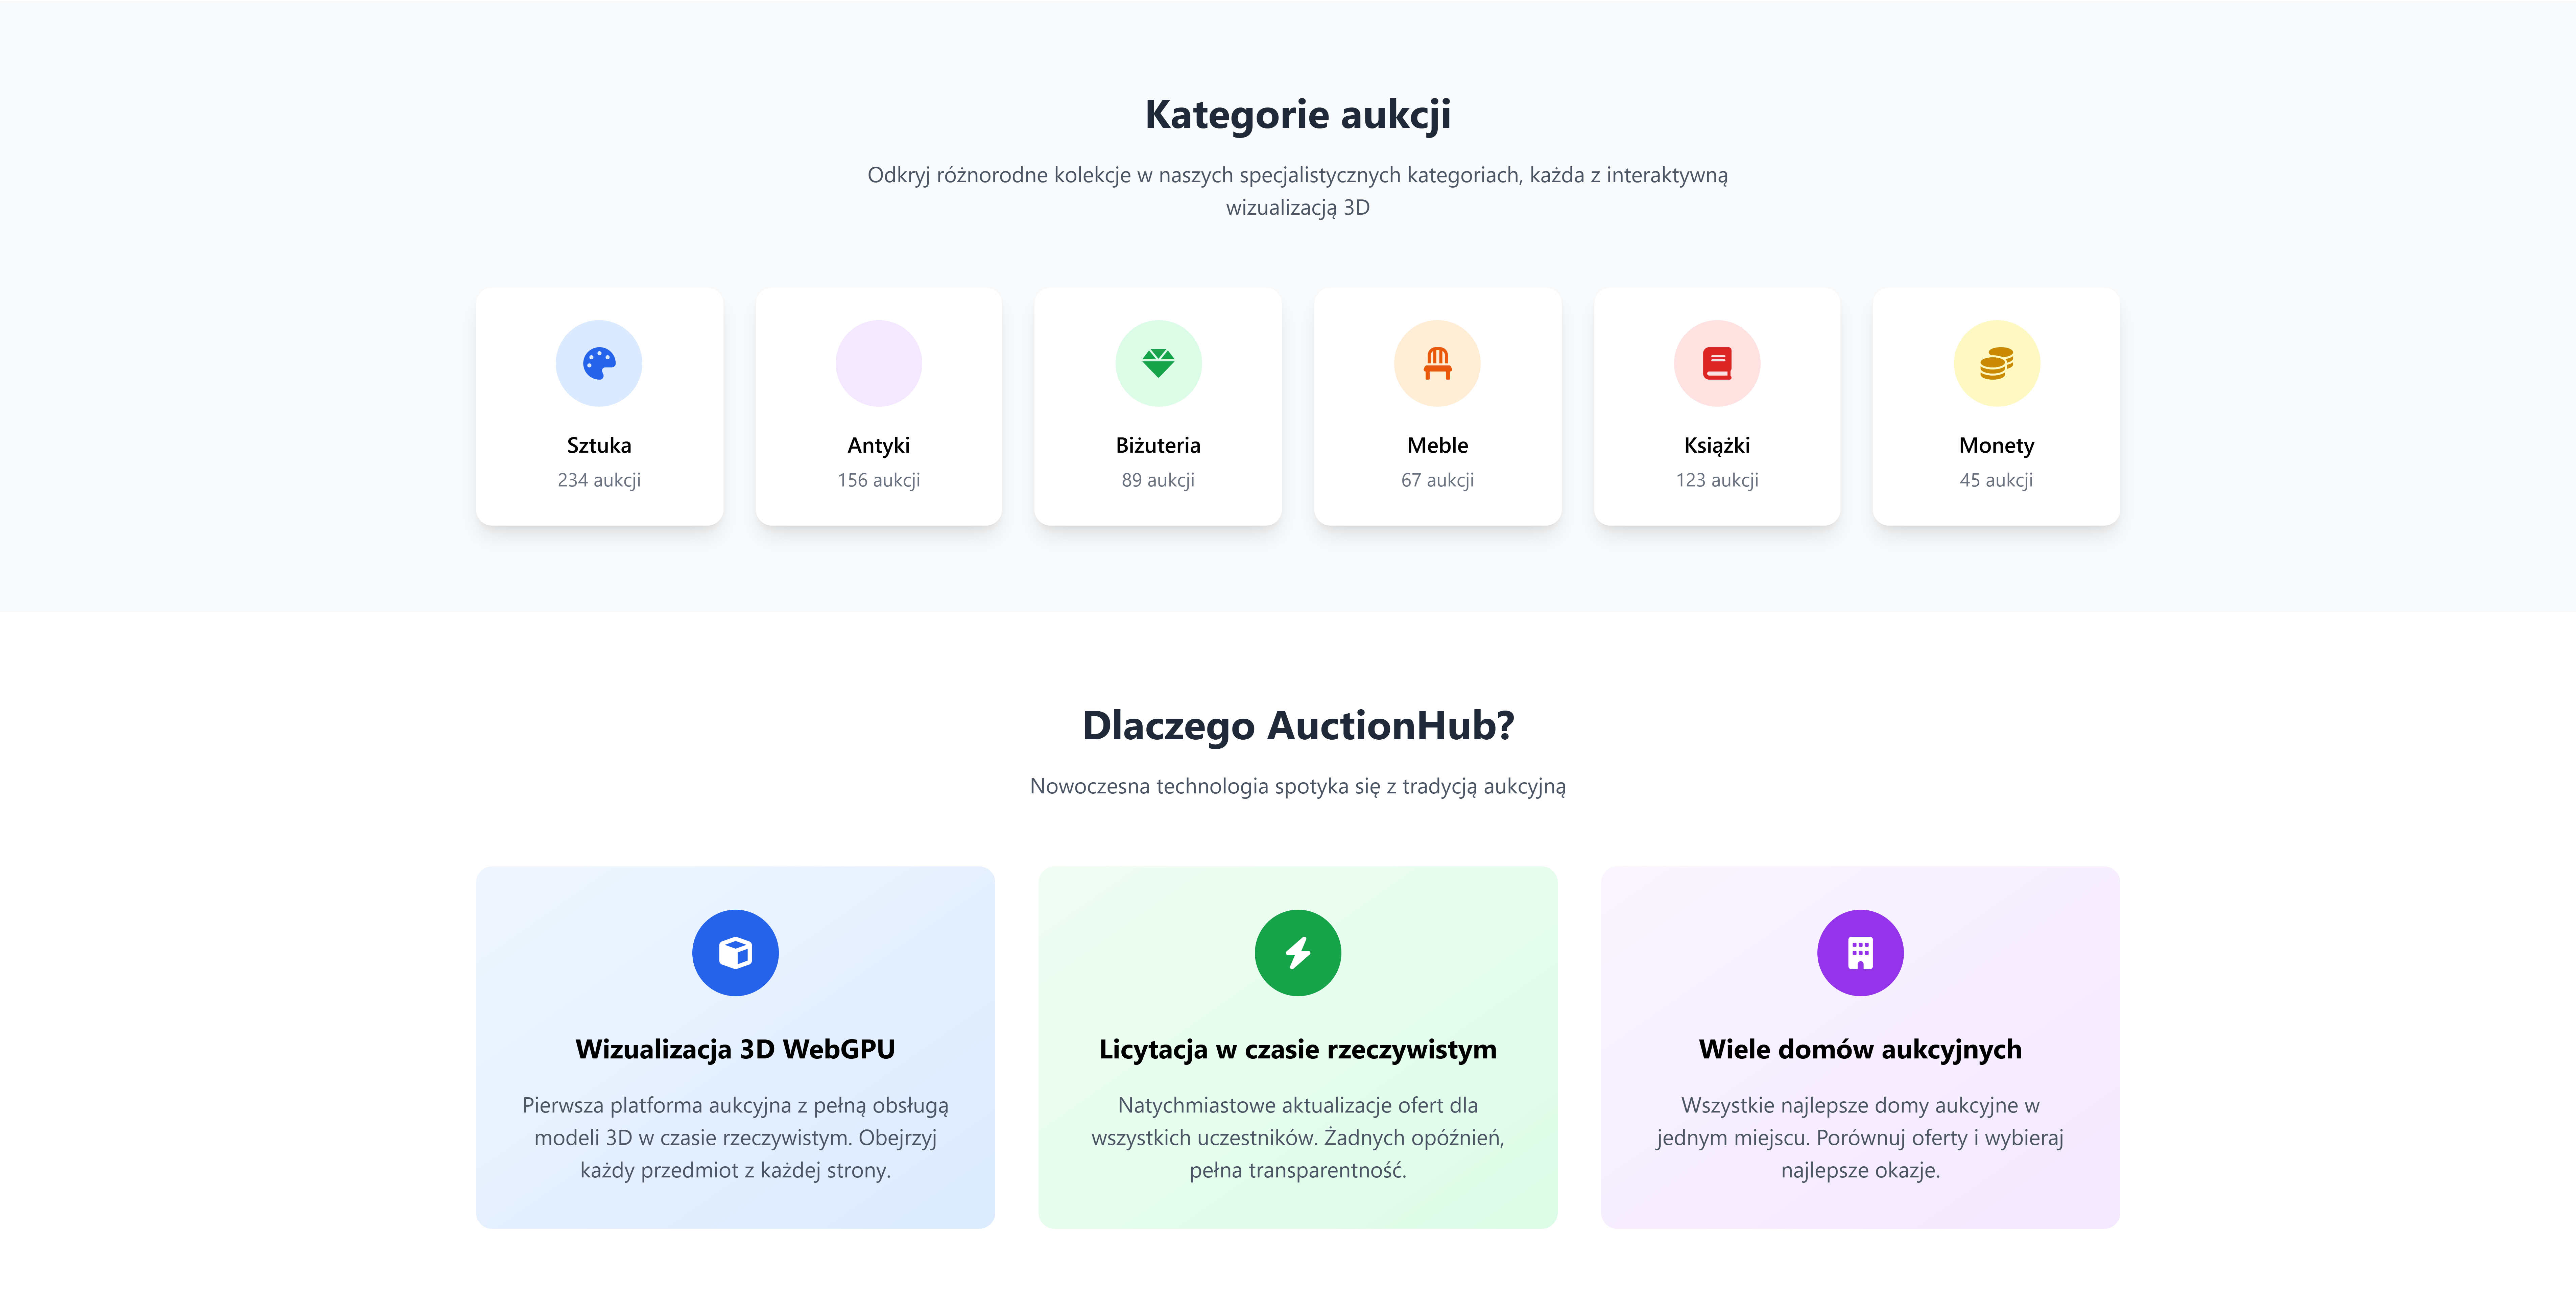
\includegraphics[
            width=\dimexpr\paperheight-2cm\relax,
            height=\dimexpr\textwidth-2cm-35.40514pt\relax,
            keepaspectratio
        ]{img/schematy/mockup-strona-glowna-2.png}
        \caption{Mockup strony głównej - widok 2}
        \label{fig:mockup2}
    \end{figure}

    \begin{figure}[p]
        \centering
        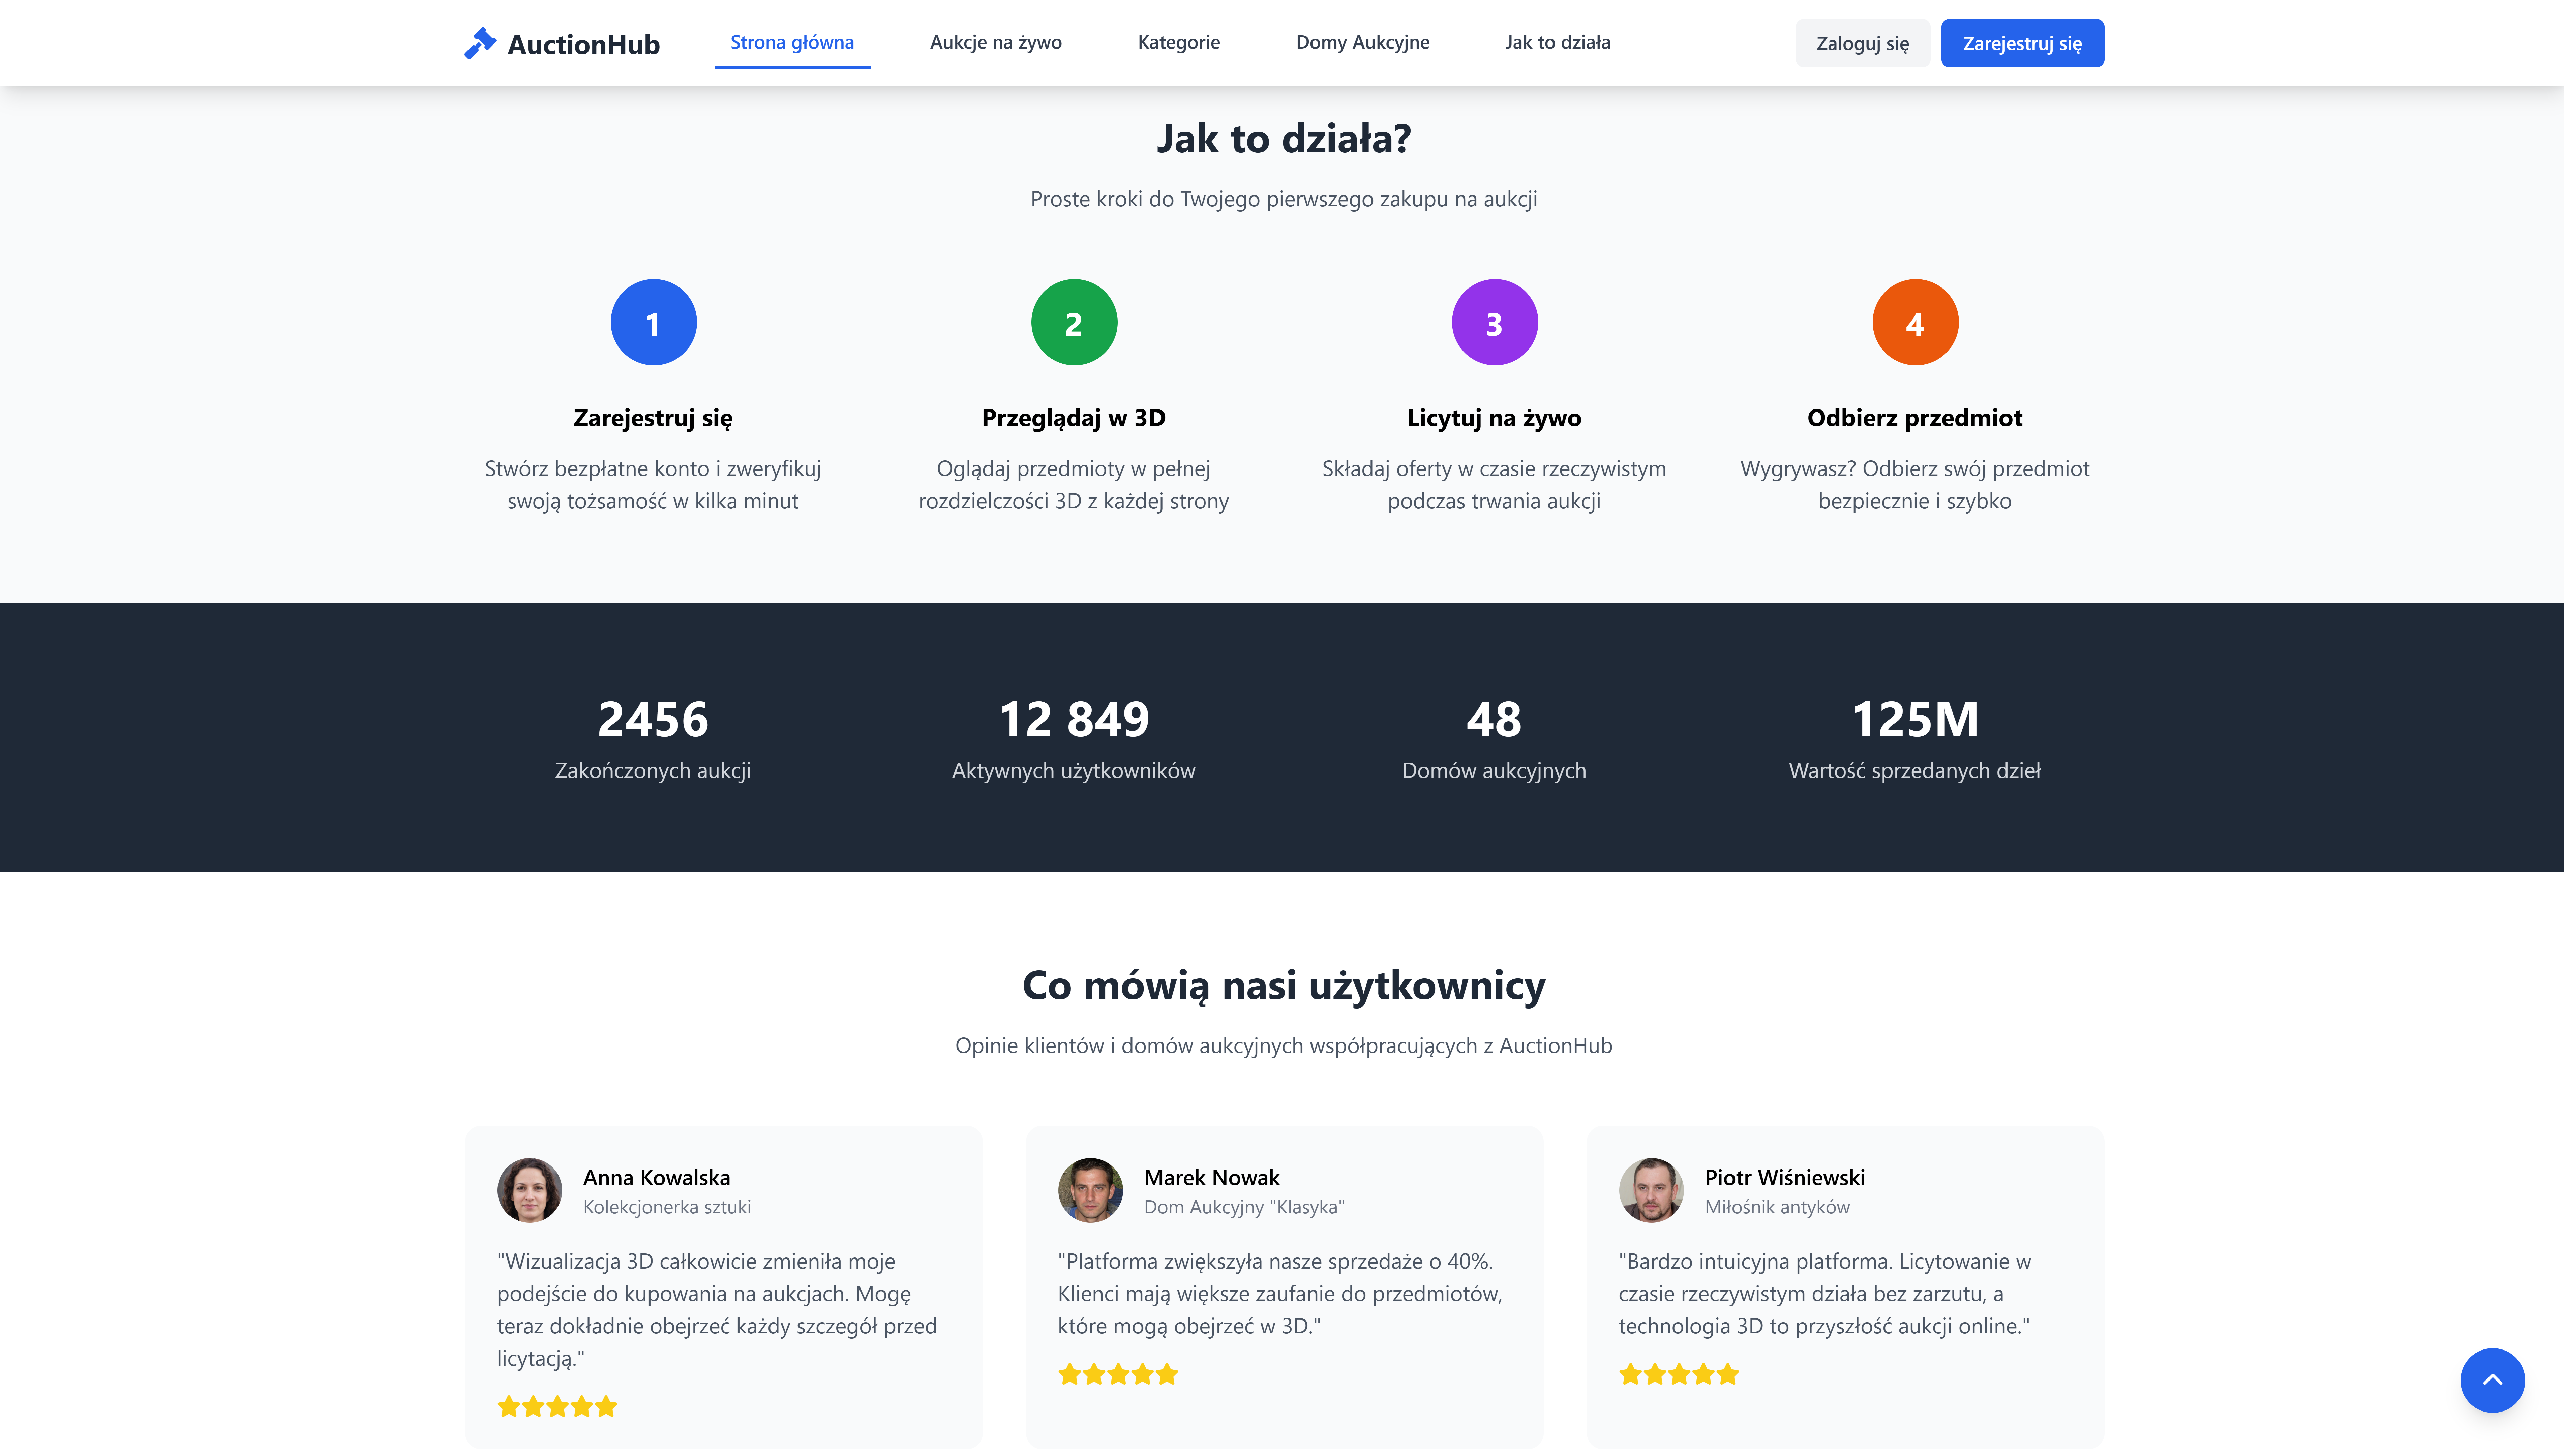
\includegraphics[
            width=\dimexpr\paperheight-2cm\relax,
            height=\dimexpr\textwidth-2cm\relax,
            keepaspectratio
        ]{img/schematy/mockup-strona-glowna-3.png}
        \caption{Mockup strony głównej - widok 3}
        \label{fig:mockup3}
    \end{figure}

    \begin{figure}[p]
        \centering
        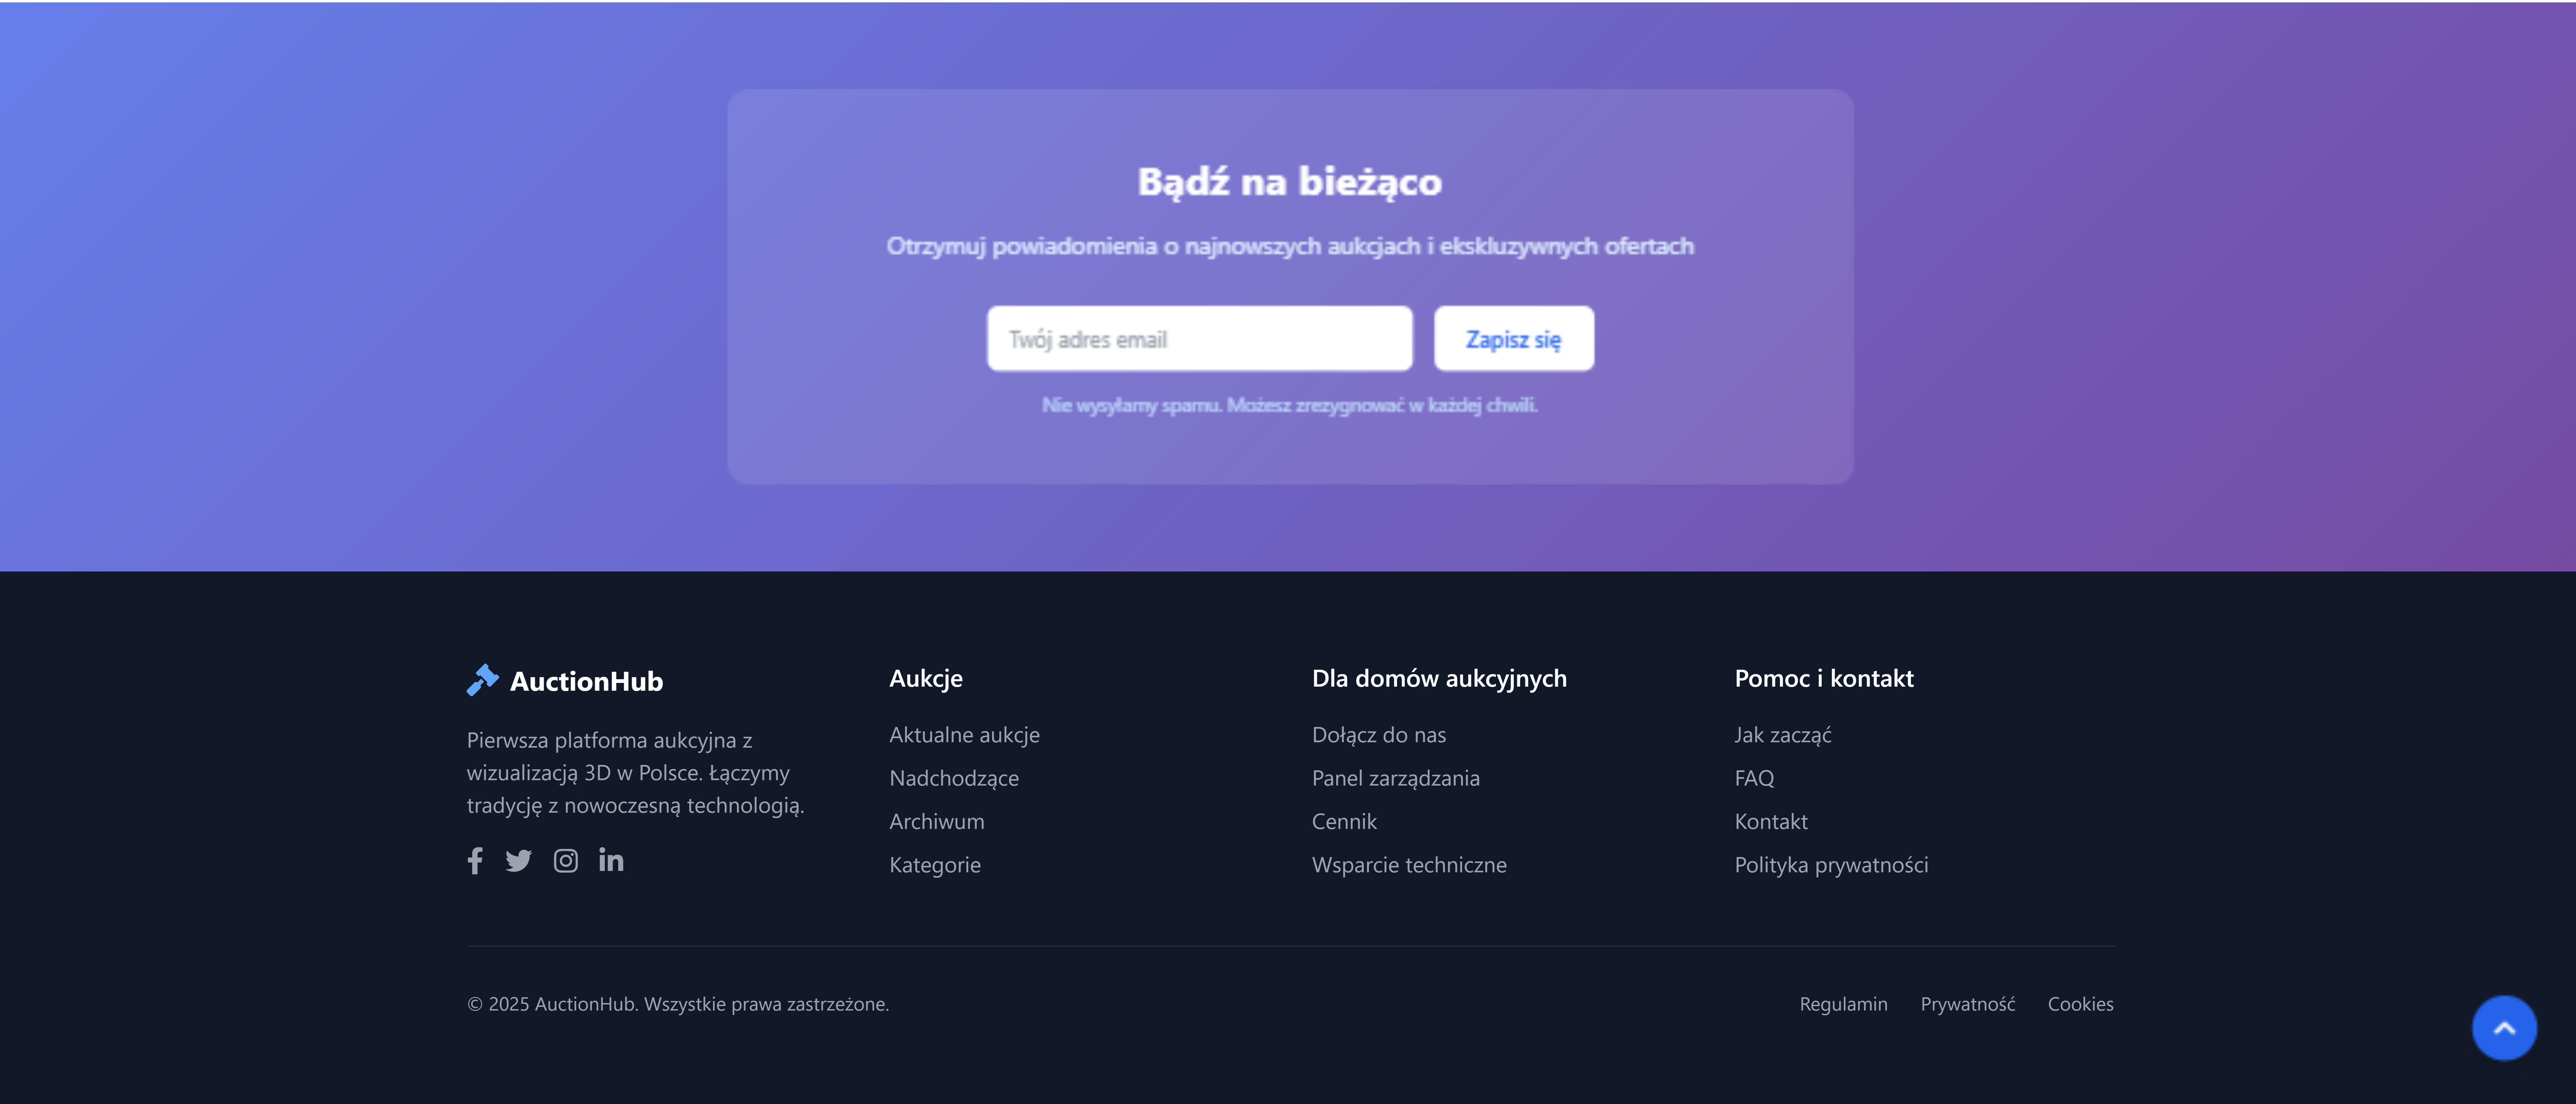
\includegraphics[
            width=\dimexpr\paperheight\relax,
            height=\dimexpr\textwidth-3.9cm-53.24414pt\relax,
            keepaspectratio
        ]{img/schematy/mockup-strona-glowna-4.png}
        \caption{Mockup strony głównej - widok 4}
        \label{fig:mockup4}
    \end{figure}

    \begin{figure}[p]
        \centering
        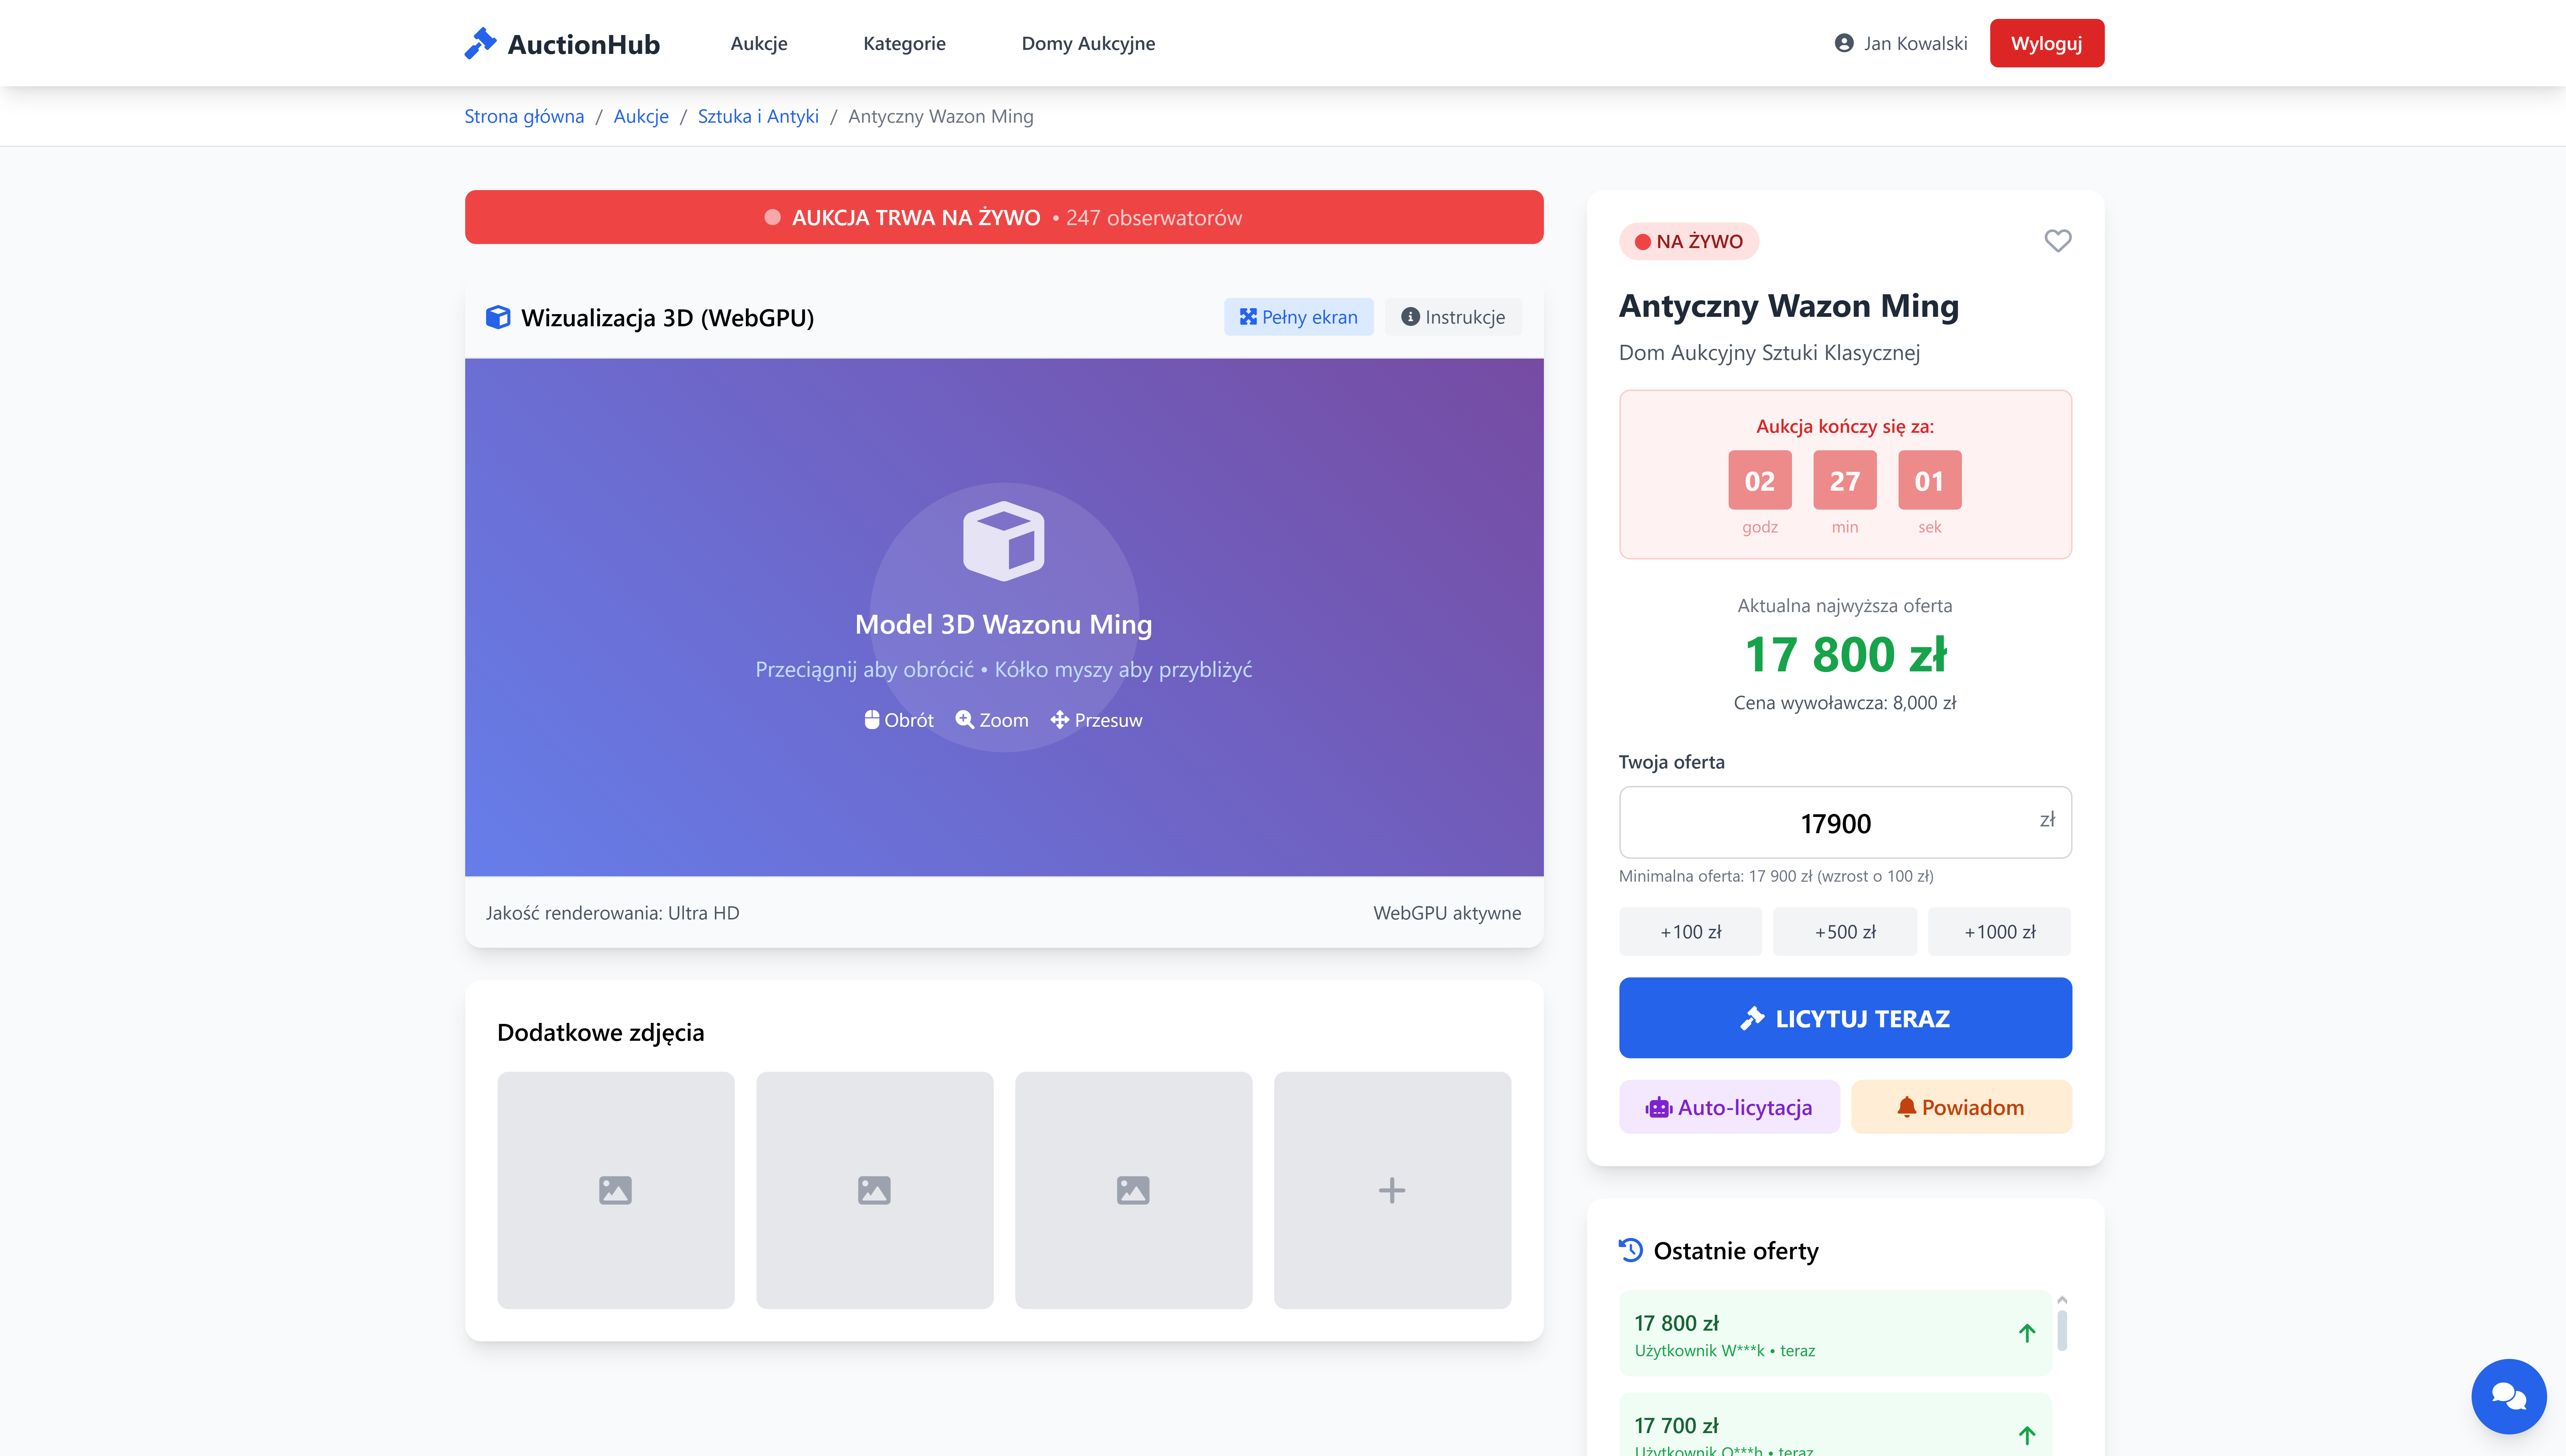
\includegraphics[
            width=\dimexpr\paperheight\relax,
            height=\dimexpr\textwidth-2cm\relax,
            keepaspectratio
        ]{img/schematy/mockup-widok-aukcji-1.png}
        \caption{Mockup widoku aukcji - widok 1}
        \label{fig:mockup5}
    \end{figure}

    \begin{figure}[p]
        \centering
        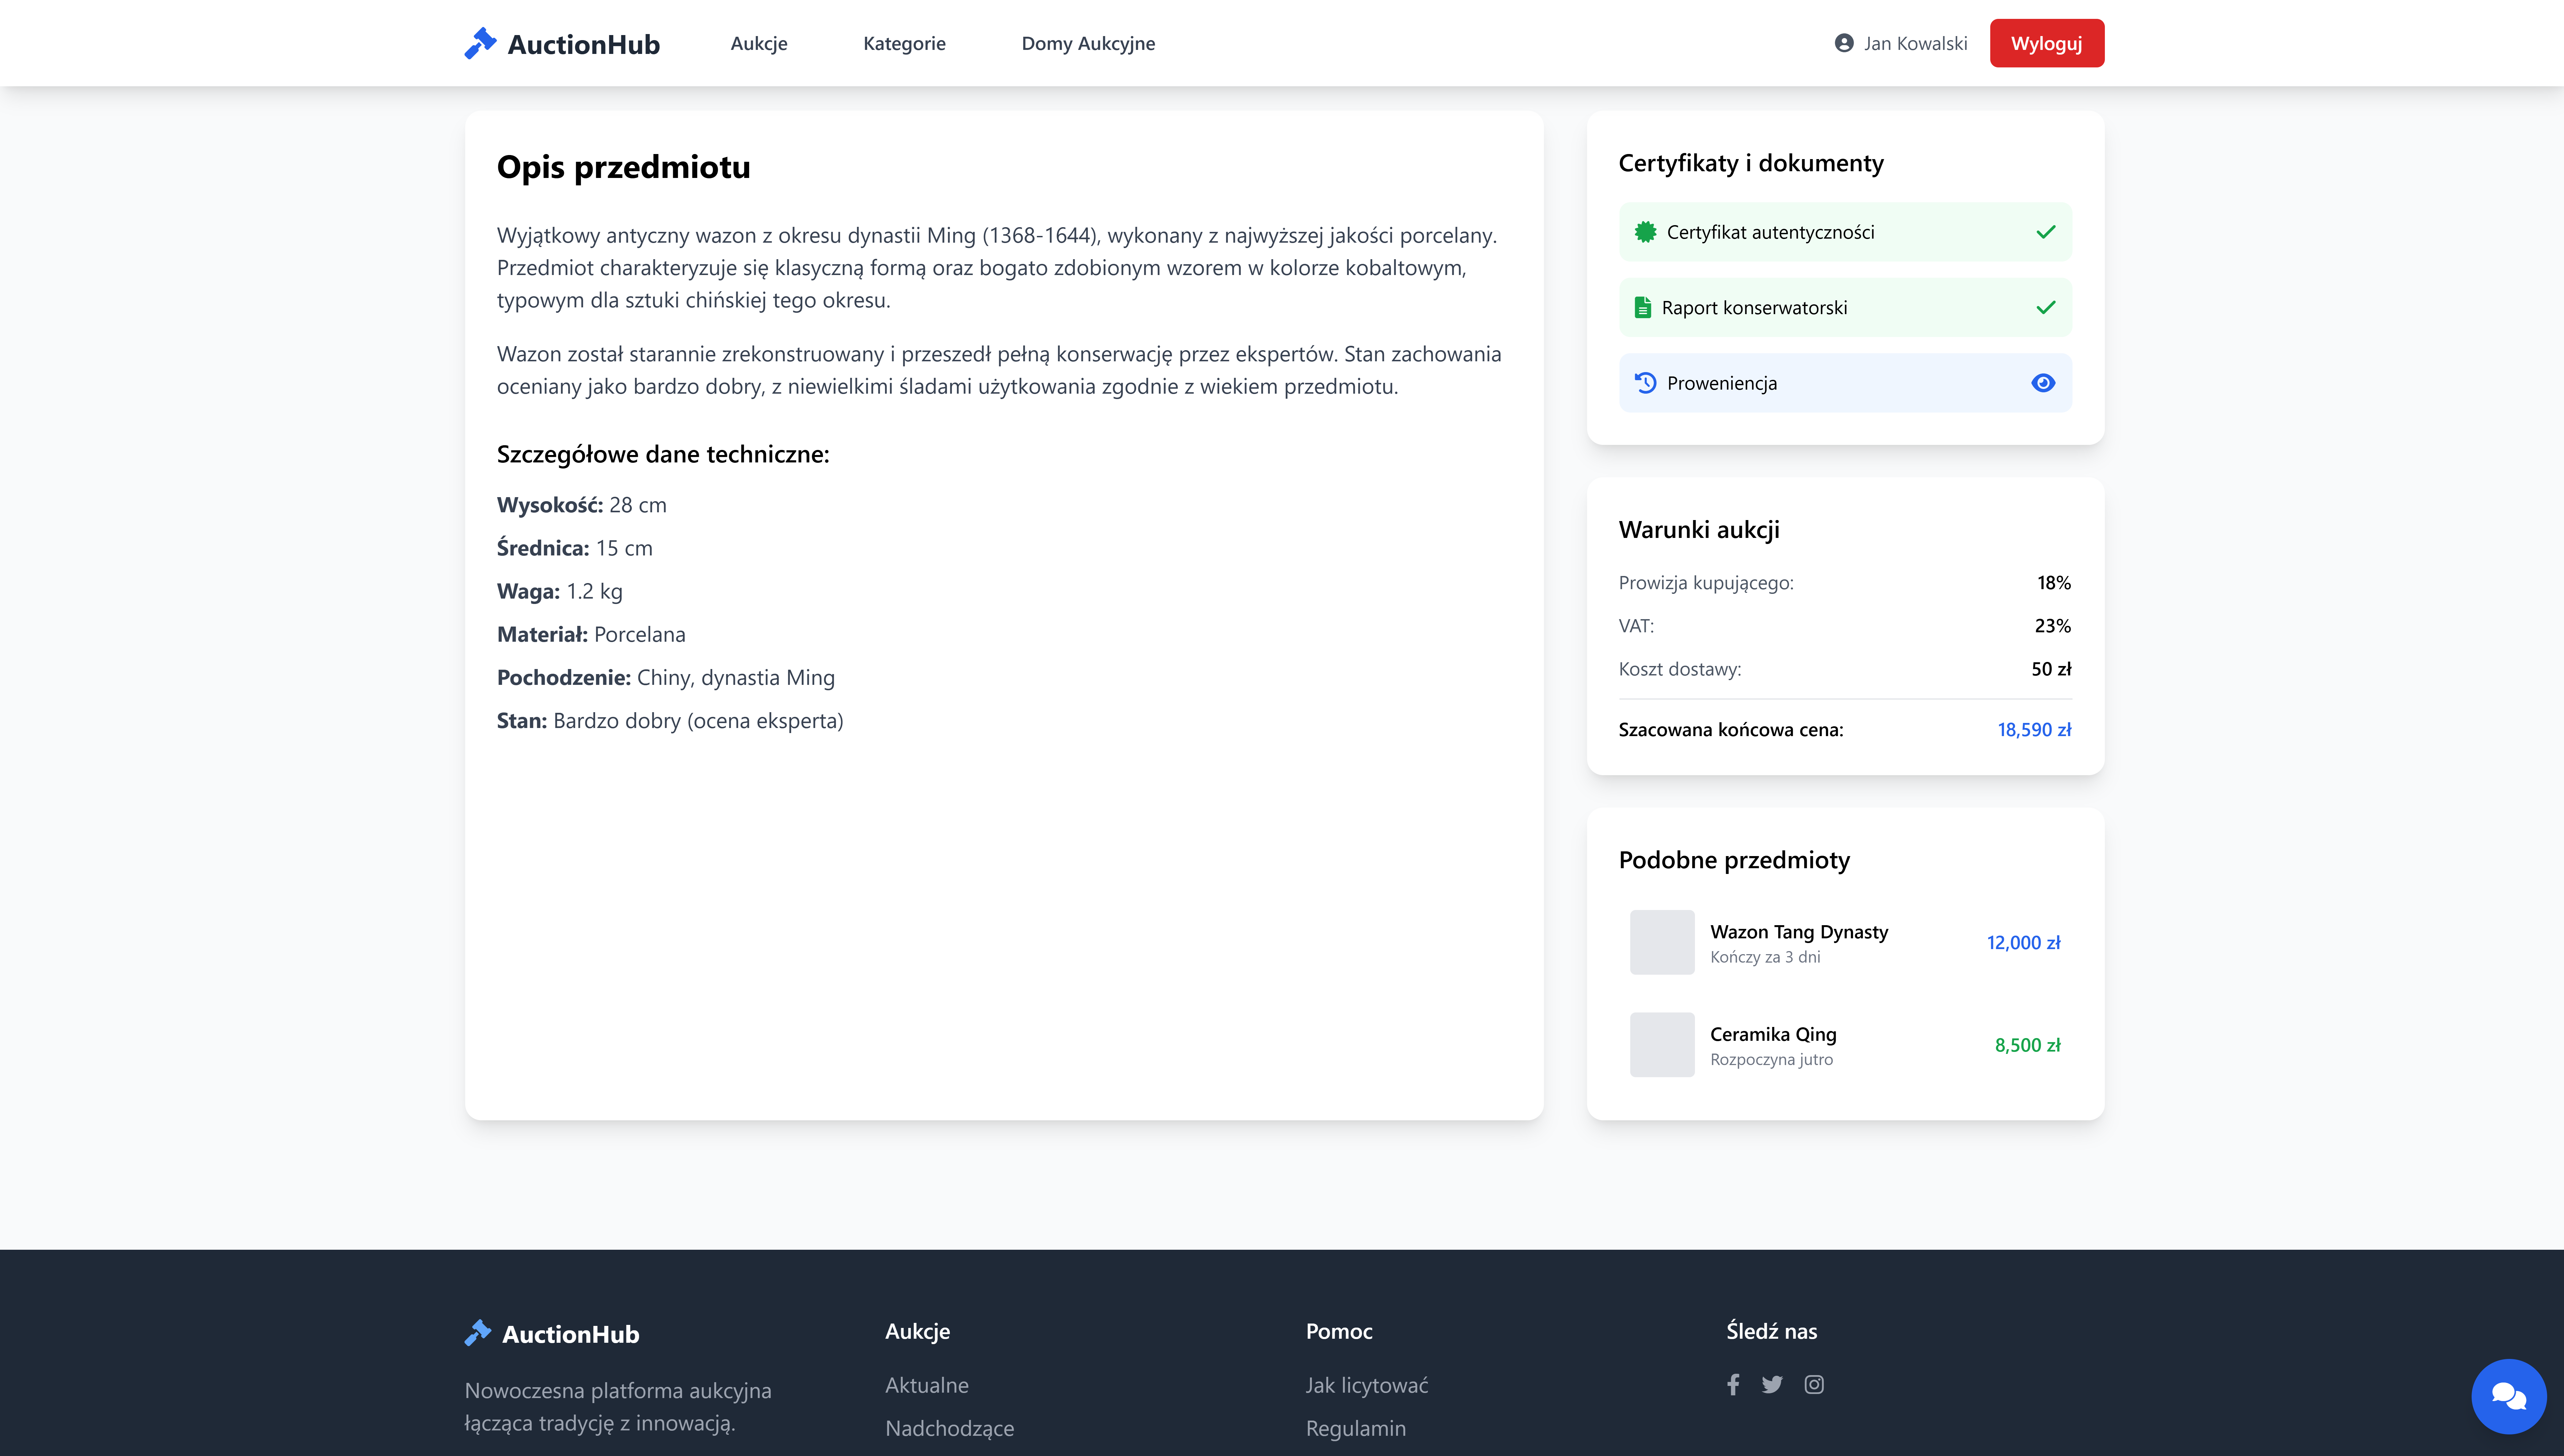
\includegraphics[
            width=\dimexpr\paperheight\relax,
            height=\dimexpr\textwidth-2cm\relax,
            keepaspectratio
        ]{img/schematy/mockup-widok-aukcji-2.png}
        \caption{Mockup widoku aukcji - widok 2}
        \label{fig:mockup6}
    \end{figure}

    \begin{figure}[p]
        \centering
        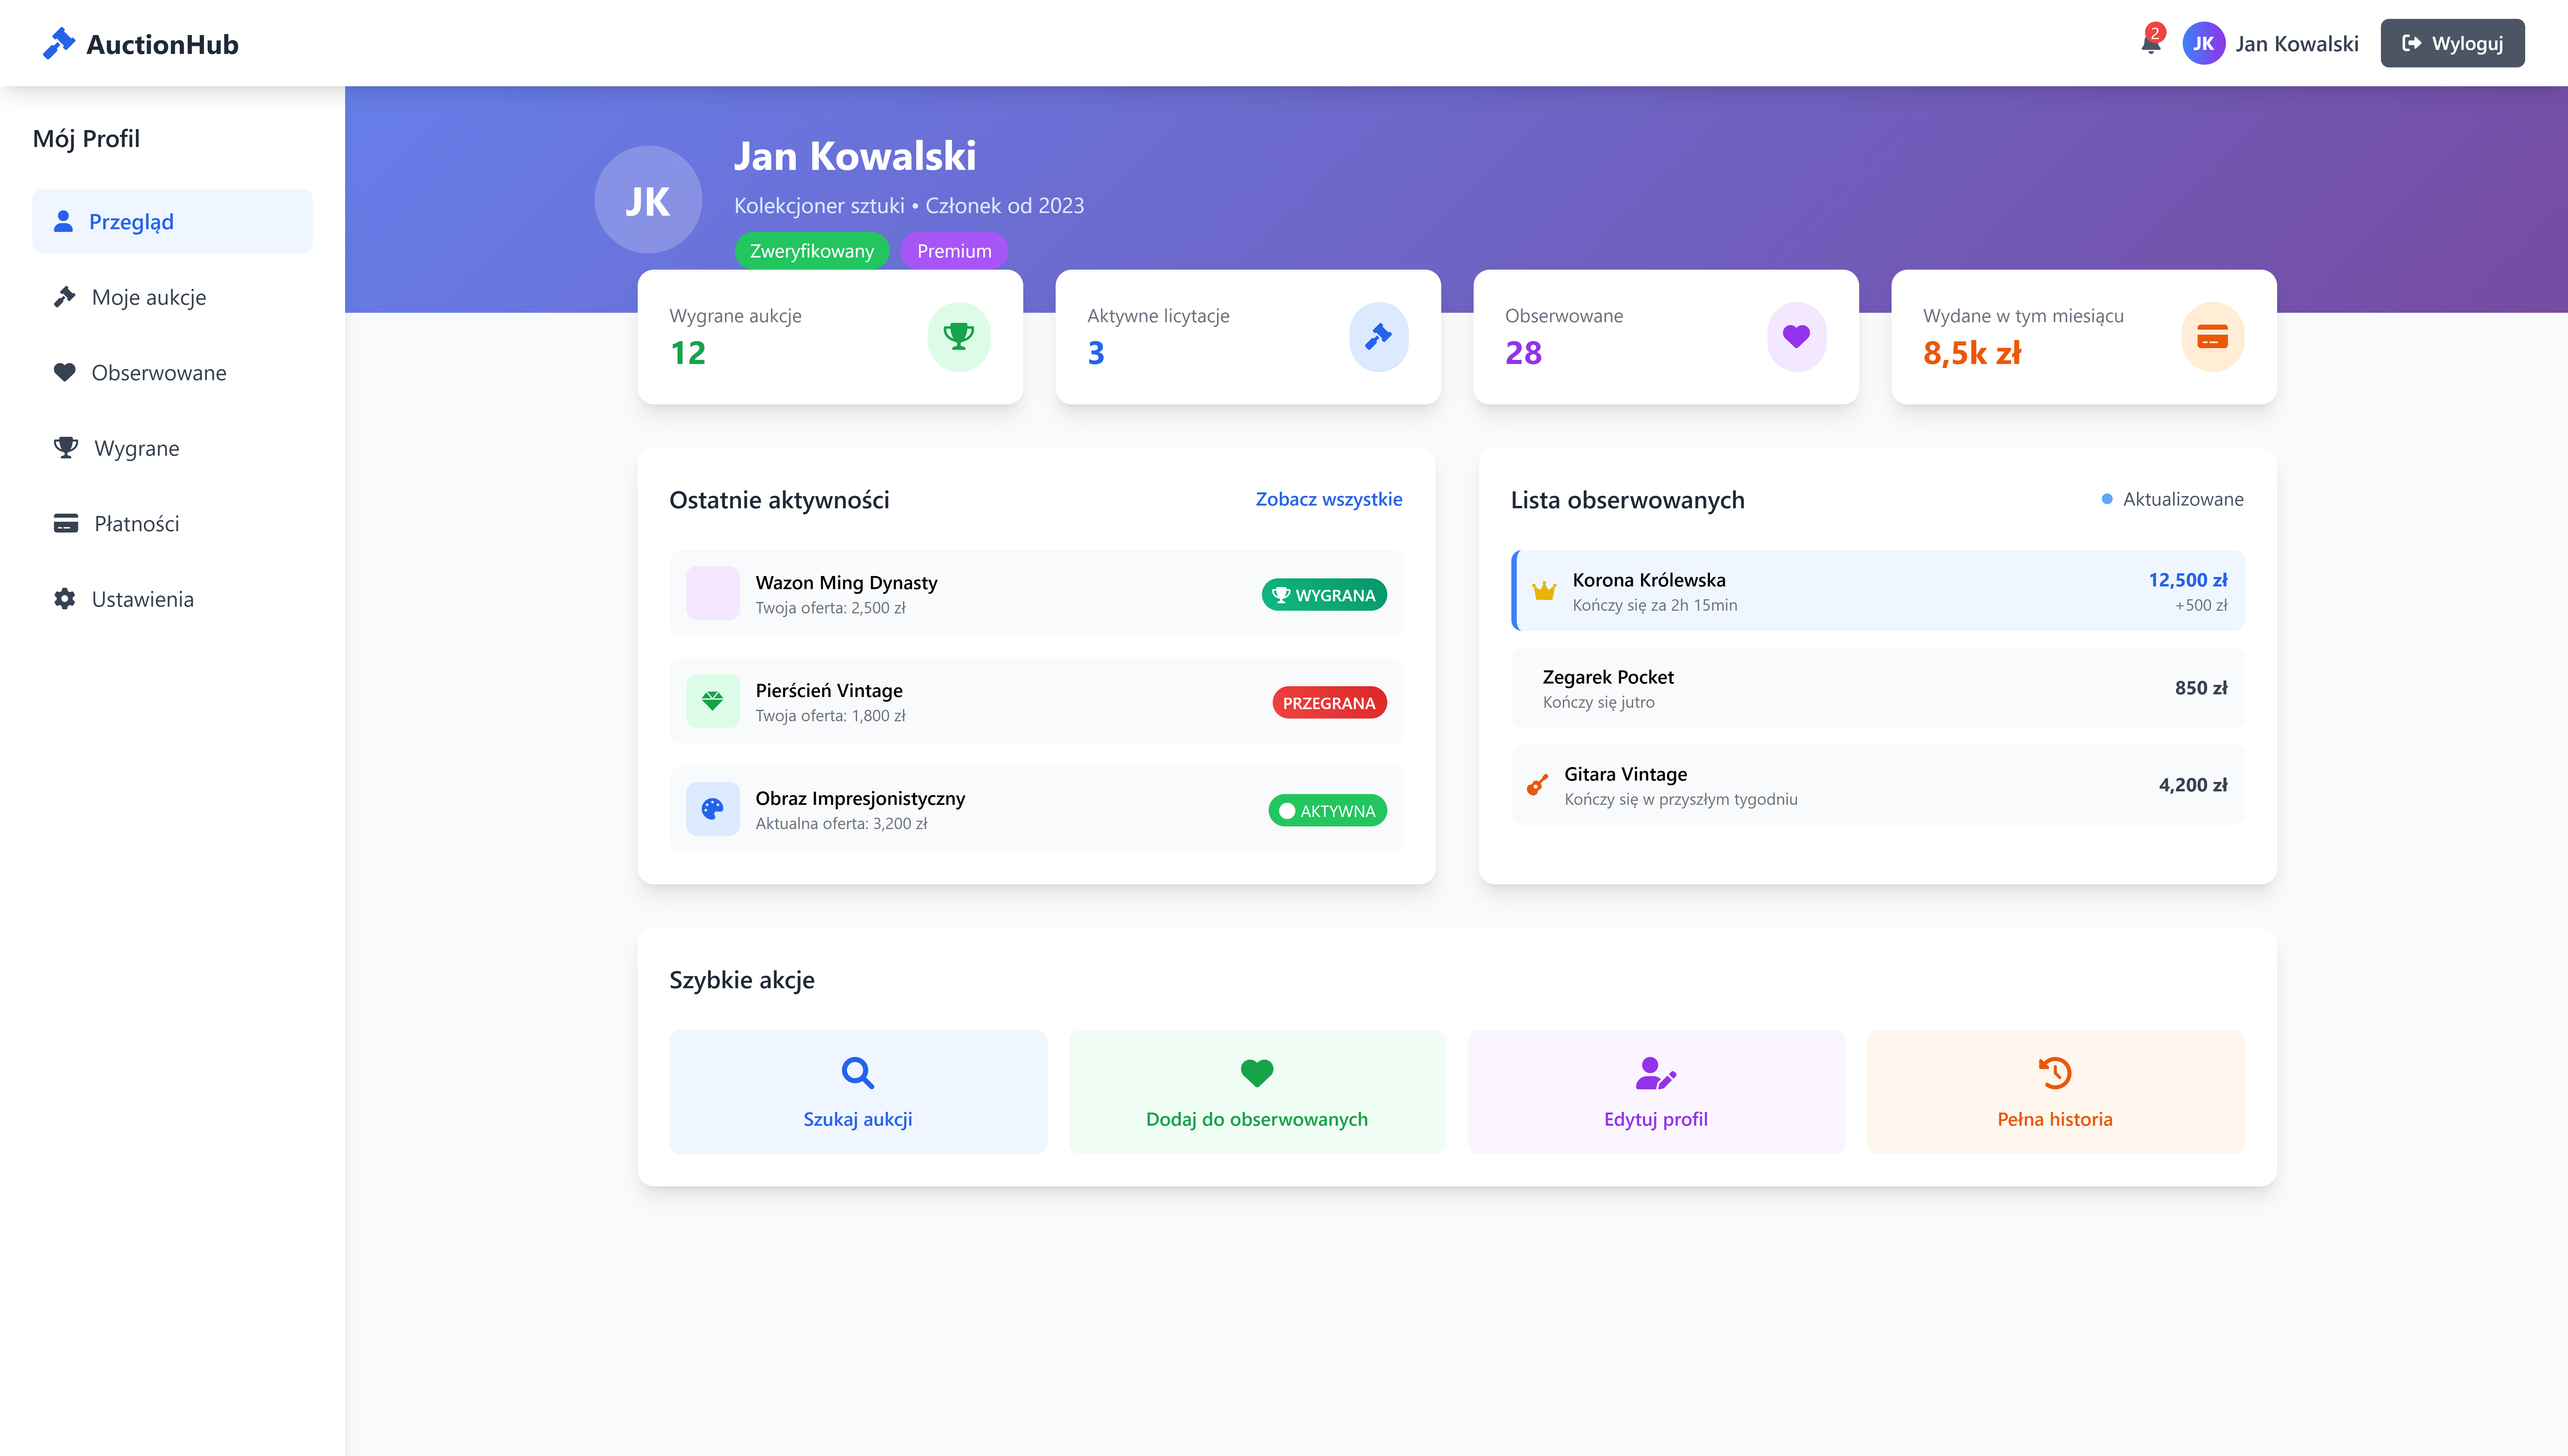
\includegraphics[
            width=\dimexpr\paperheight\relax,
            height=\dimexpr\textwidth-2cm\relax,
            keepaspectratio
        ]{img/schematy/mockup-panel-user.png}
        \caption{Mockup widoku panelu urzytkownika}
        \label{fig:mockup7}
    \end{figure}

    \begin{figure}[p]
        \centering
        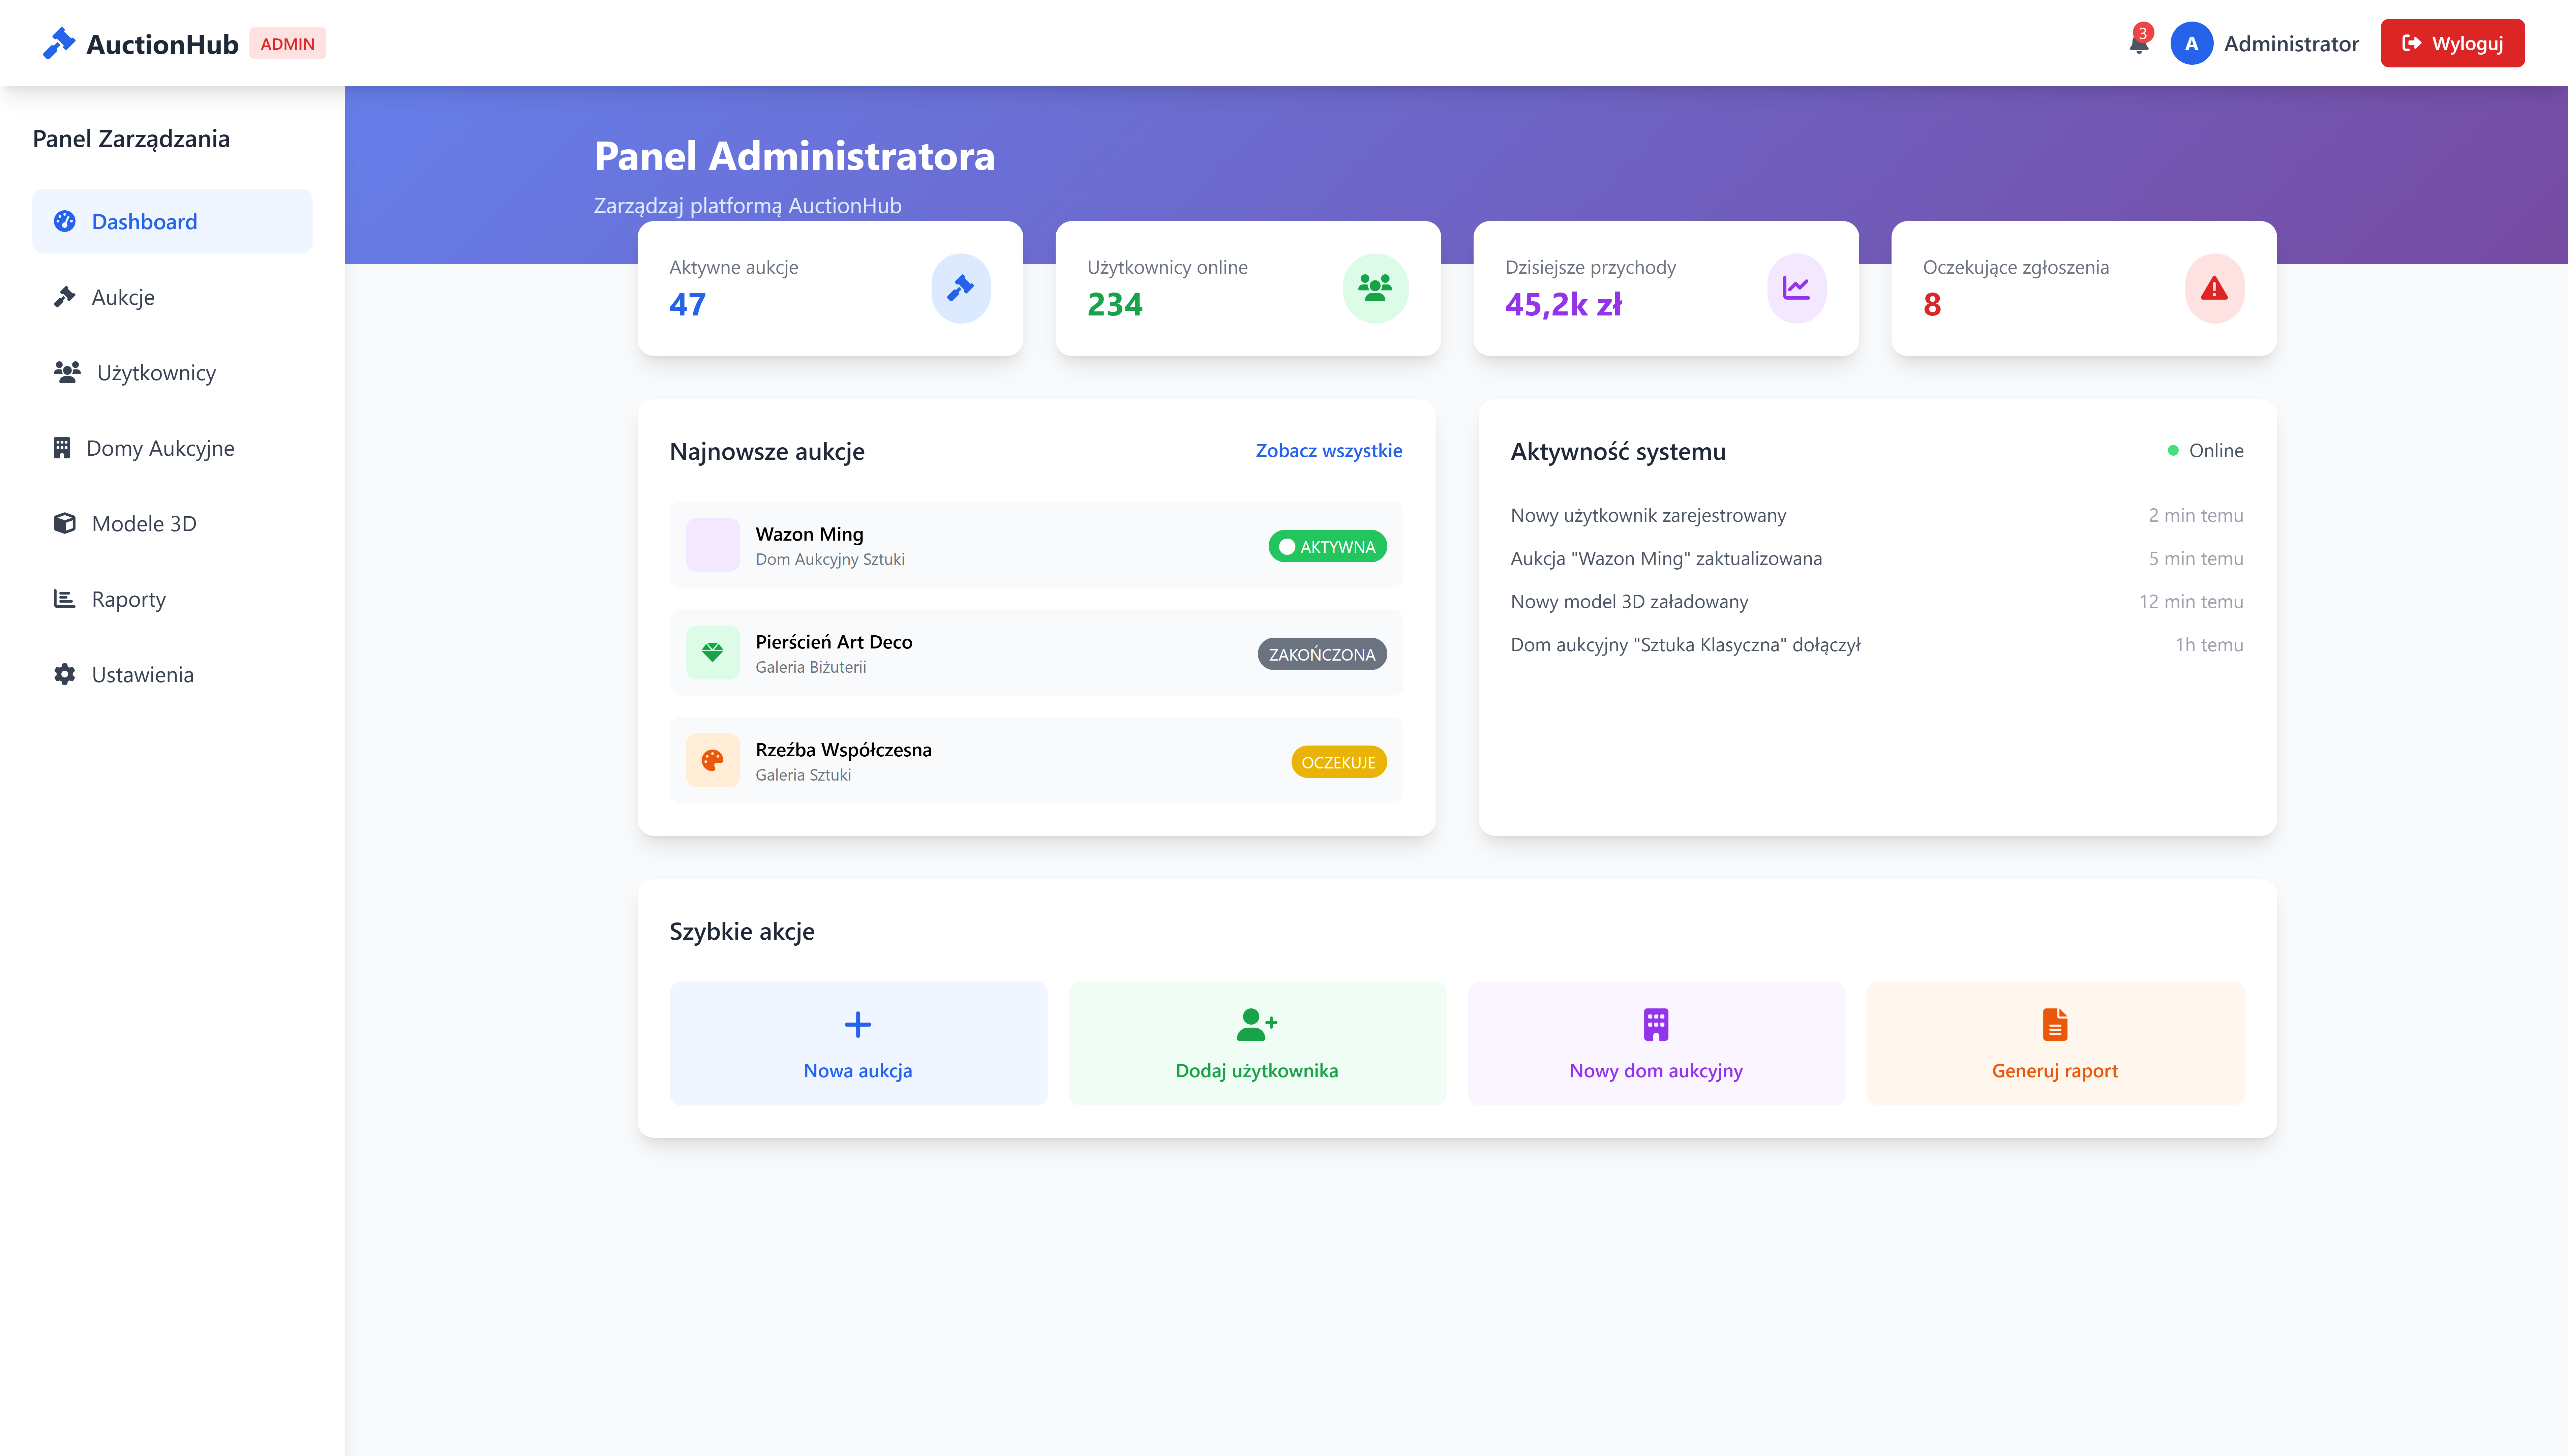
\includegraphics[
            width=\dimexpr\paperheight\relax,
            height=\dimexpr\textwidth-2cm\relax,
            keepaspectratio
        ]{img/schematy/mockup-panel-admin.png}
        \caption{Mockup widoku panelu administratora}
        \label{fig:mockup8}
    \end{figure}
\end{landscape}

\subsection{Model danych}
Poniższe diagramy klas prezentują model danych systemu aukcyjnego z kluczowymi encjami (Użytkownik, Aukcja, Przedmiot, PozycjaAukcji, Oferta) oraz ich relacjami; uproszczony diagram pokazuje jedynie nazwy klas i powiązania, a rozszerzony zawiera szczegółowe atrybuty i typy.
\begin{figure}[htbp]
    \centering
    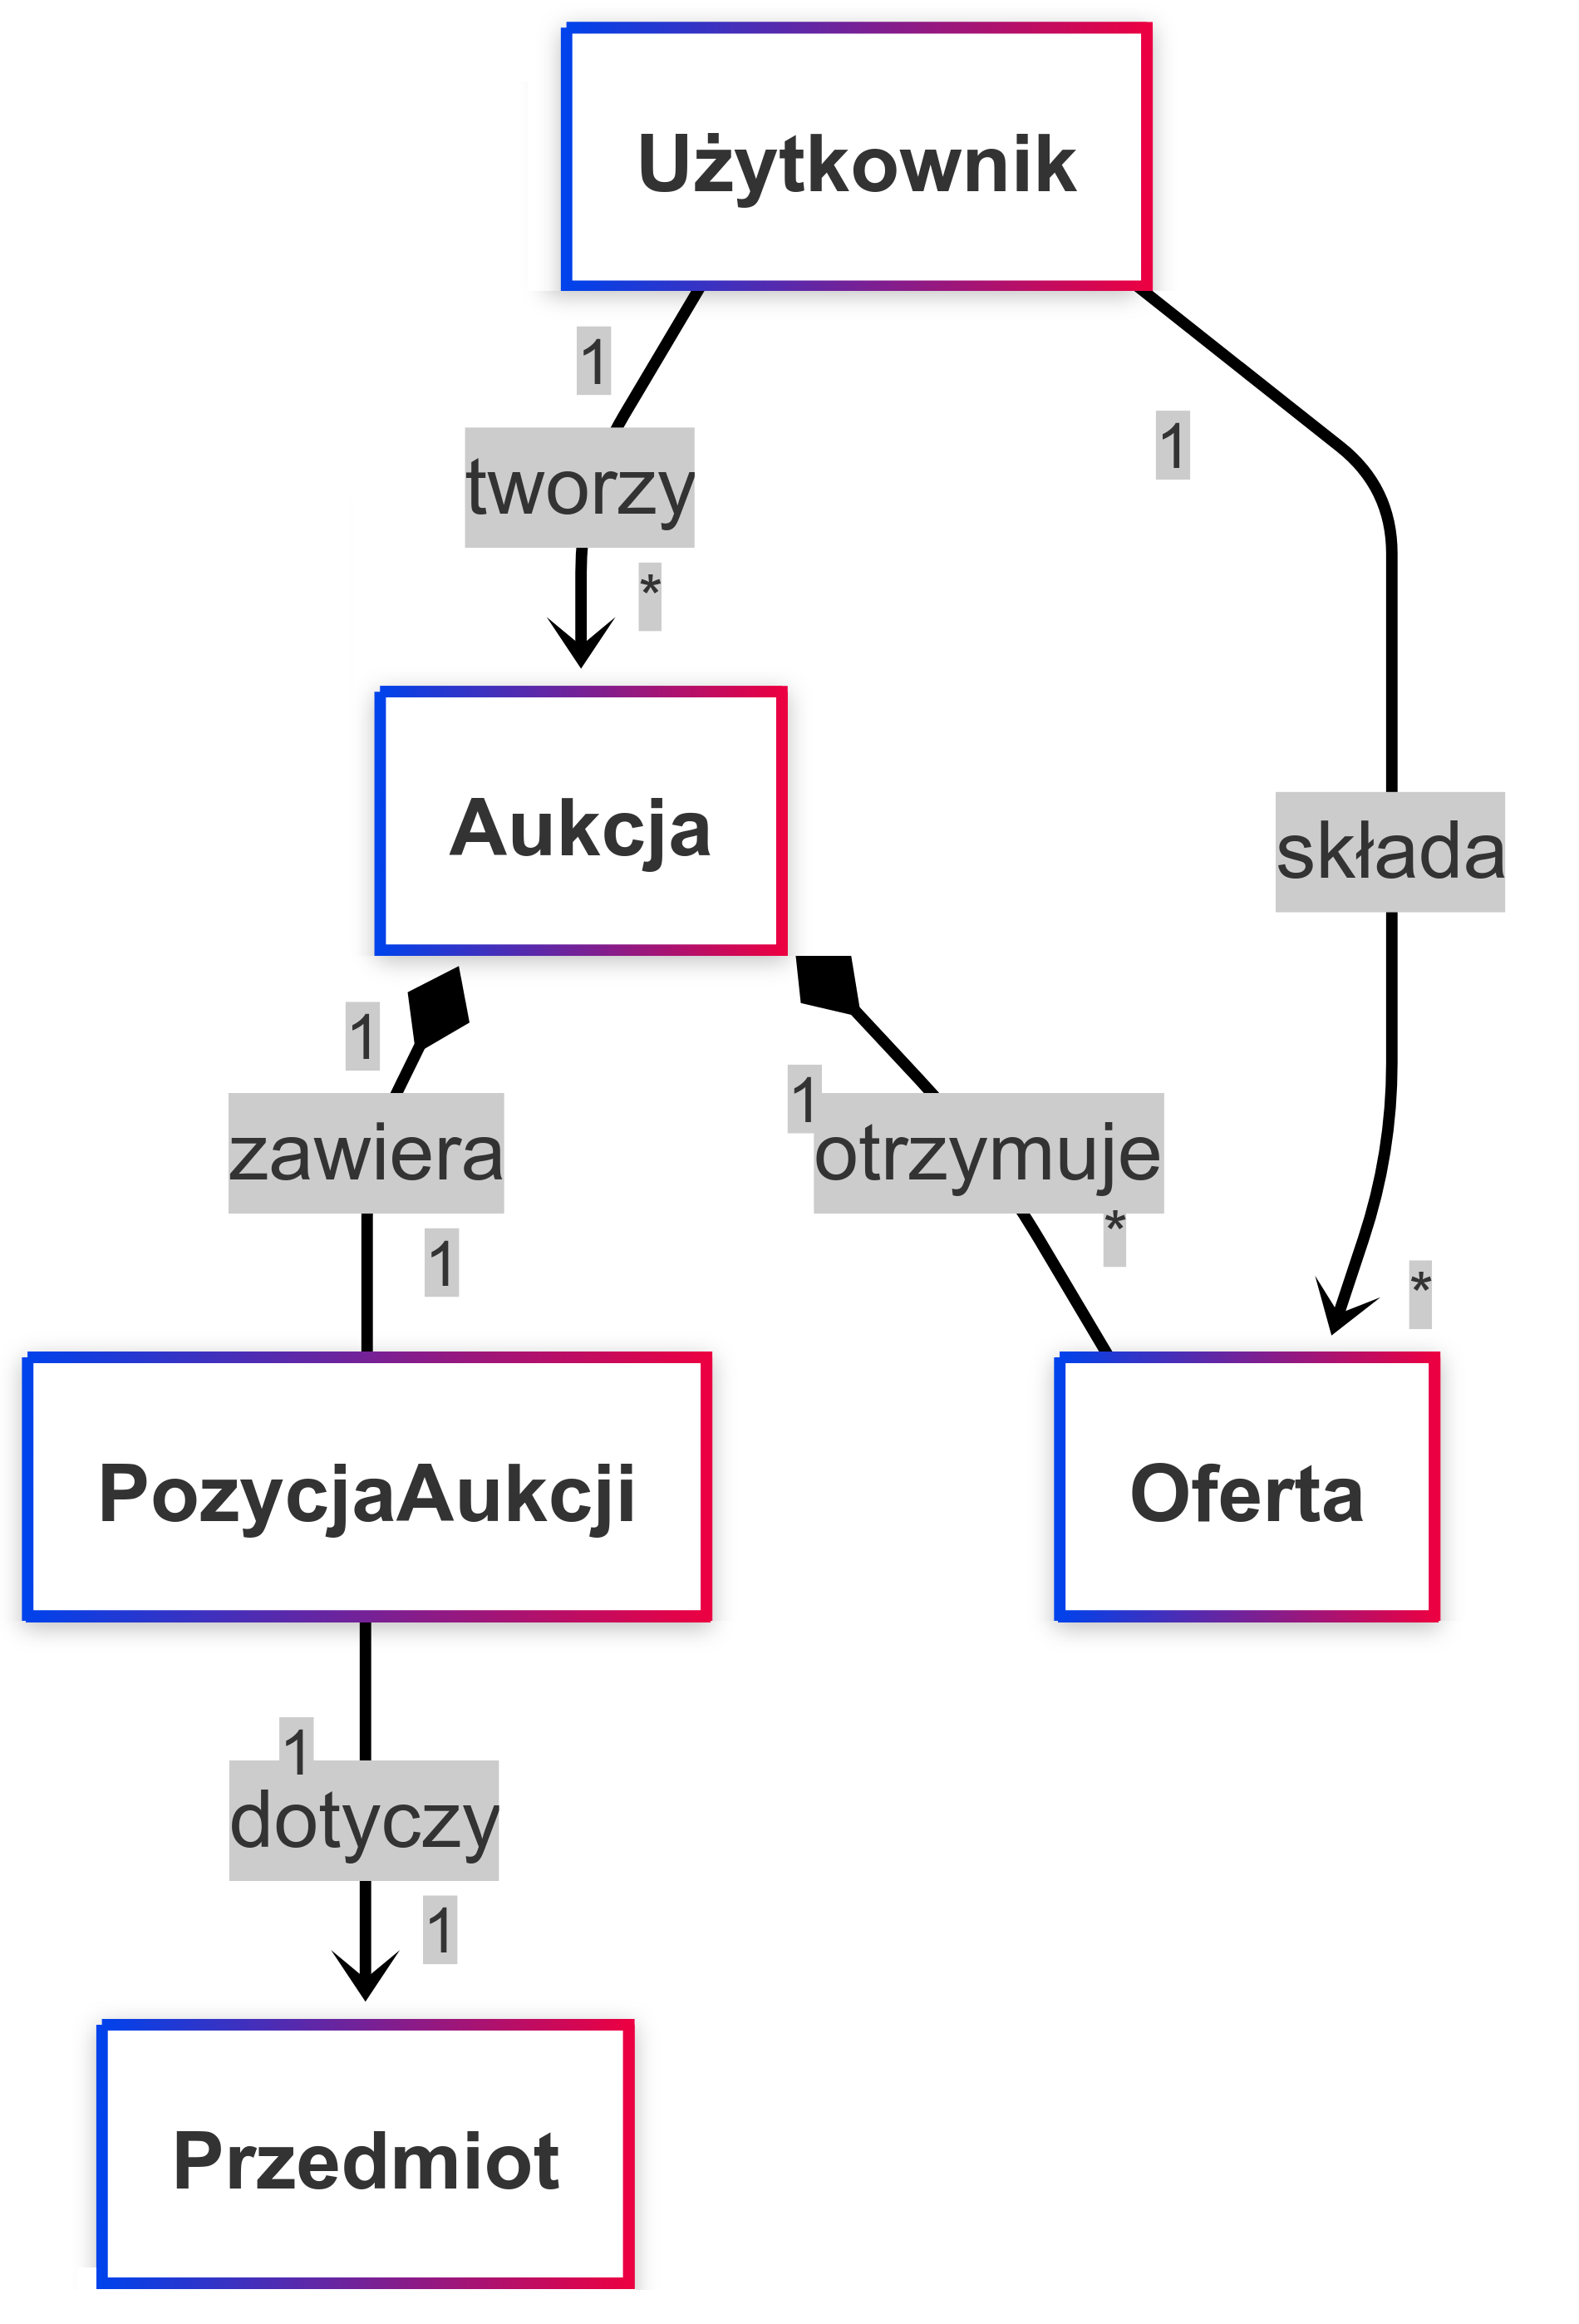
\includegraphics[
        width=\dimexpr\textwidth-5cm\relax,
        height=\dimexpr\paperheight-2cm\relax,
        keepaspectratio
    ]{img/schematy/model-danych-prosty.png}
    \caption{Model danych - uproszczony diagram klas}
    \label{fig:zdj19}
\end{figure}

\begin{figure}[htbp]
    \centering
    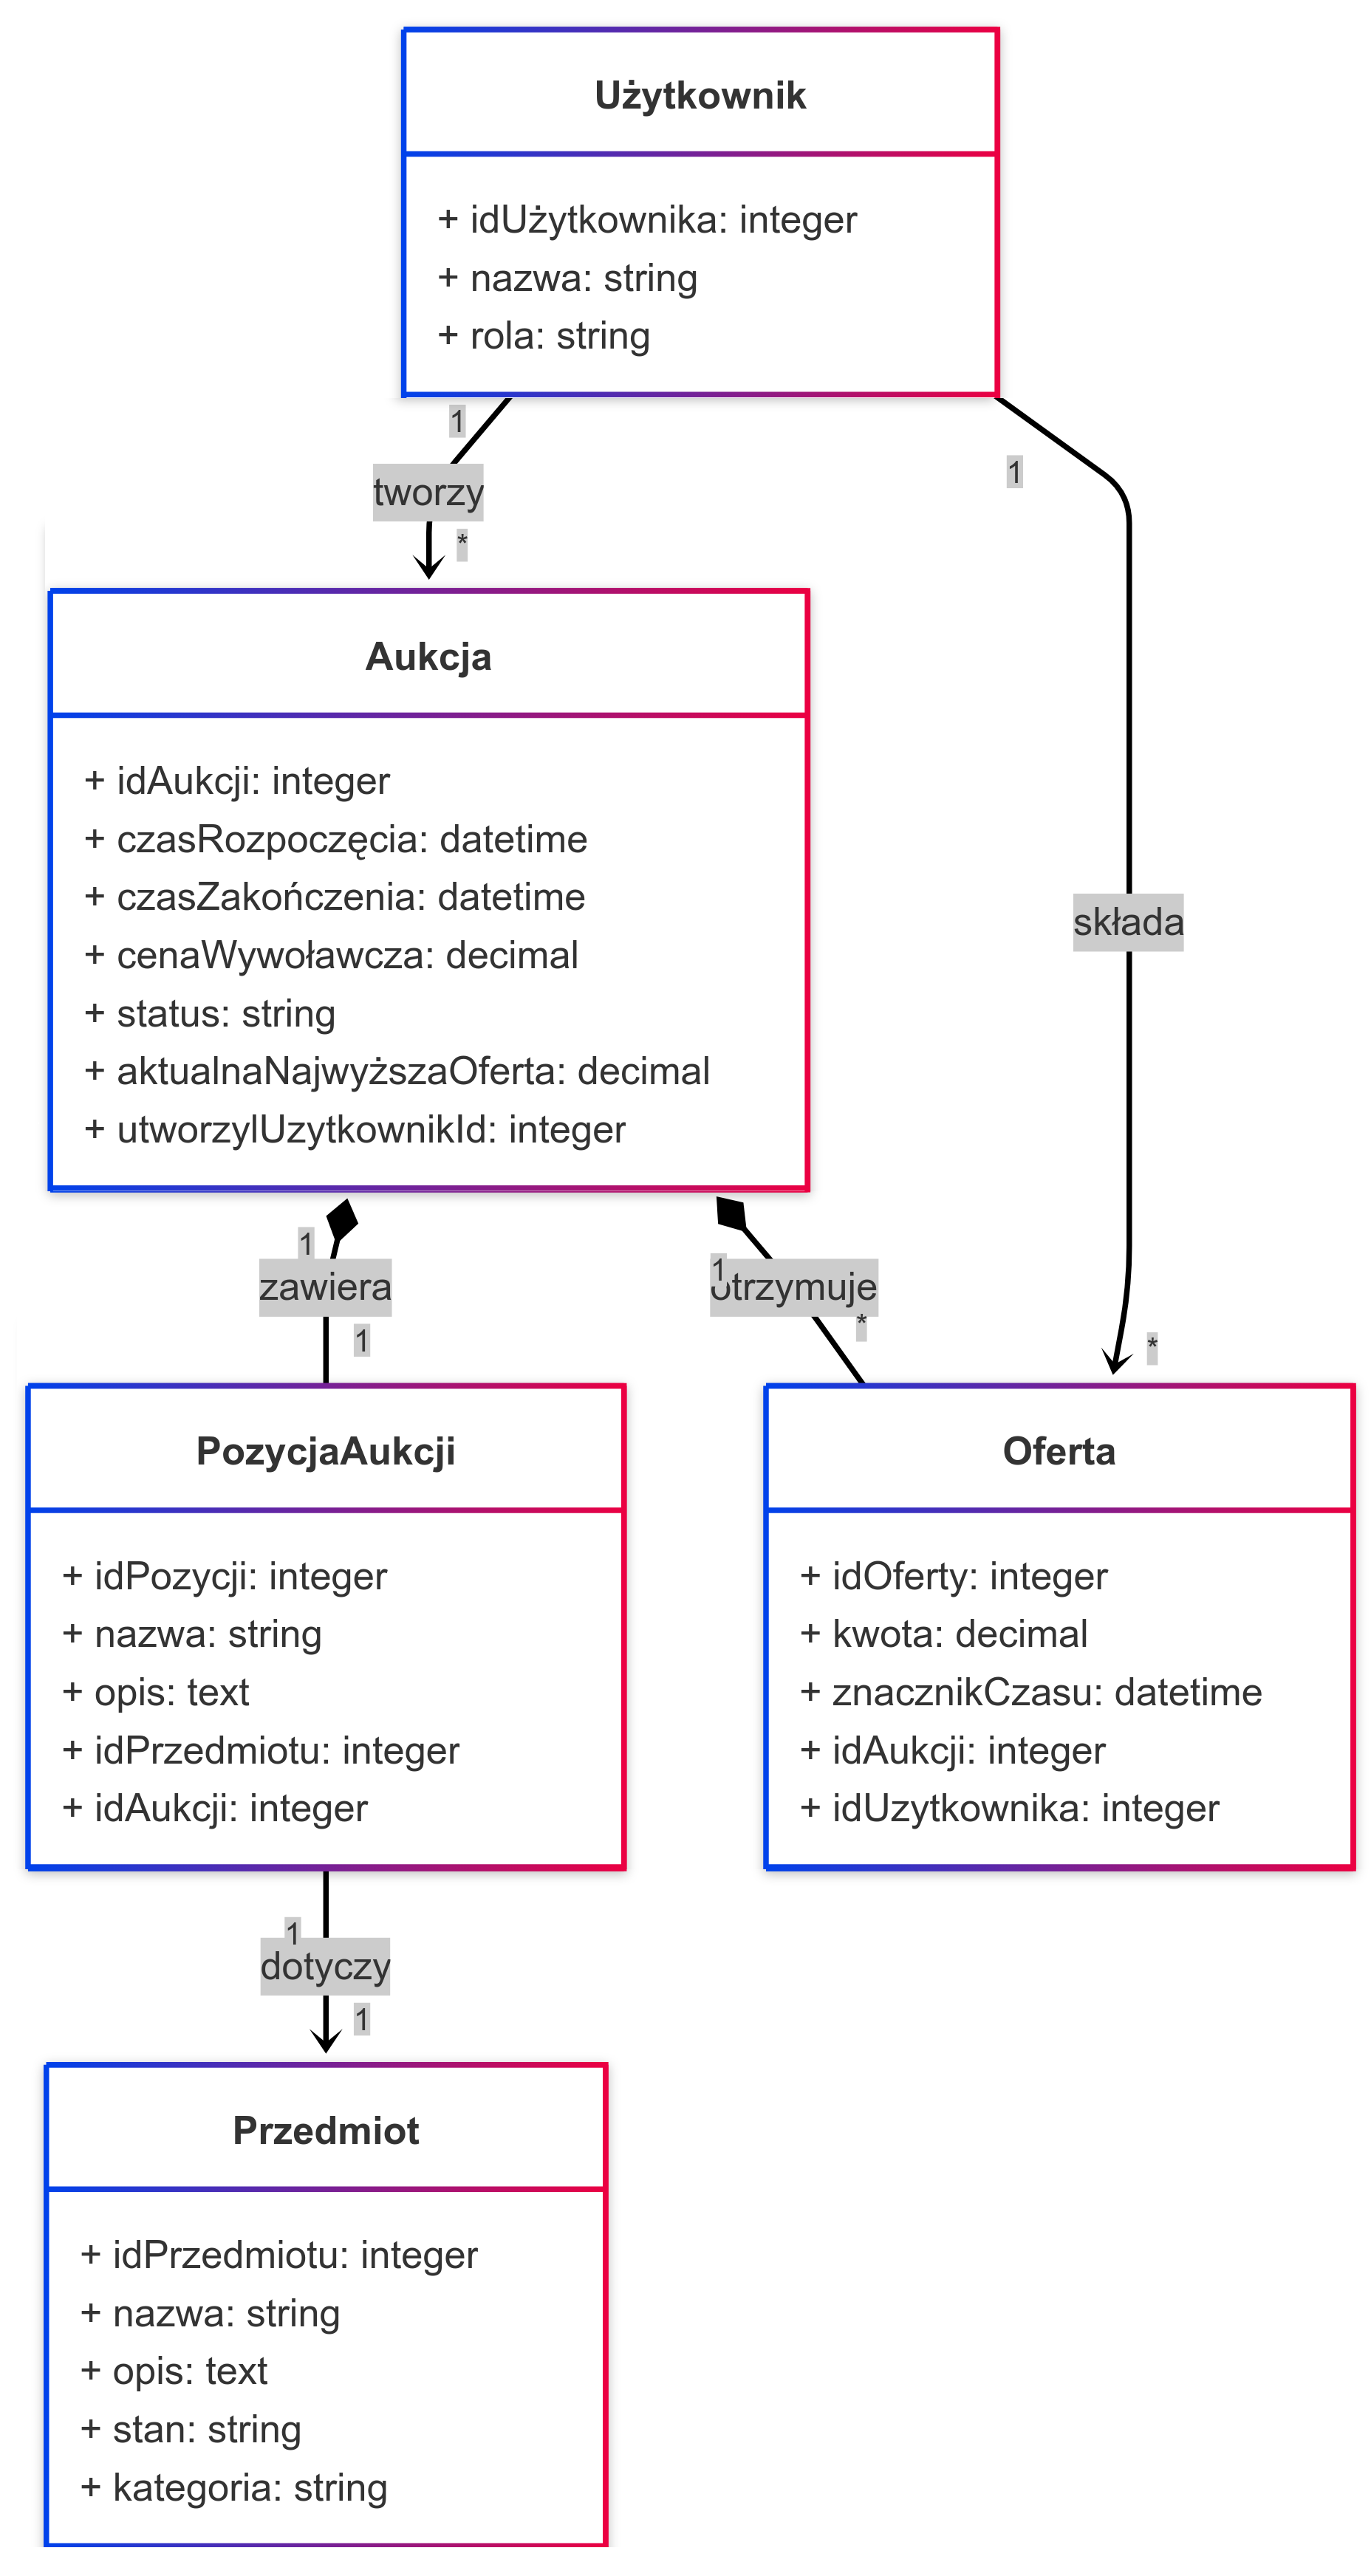
\includegraphics[
        width=\dimexpr\textwidth-3cm\relax,
        height=\dimexpr\paperheight-2cm\relax,
        keepaspectratio
    ]{img/schematy/model-danych-krzywy.png}
    \caption{Model danych - rozszerzony diagram klas}
    \label{fig:zdj20}
\end{figure}